\documentclass[11pt]{article}

    \usepackage[breakable]{tcolorbox}
    \usepackage{parskip} % Stop auto-indenting (to mimic markdown behaviour)

    \usepackage{iftex}
    \ifPDFTeX
    	\usepackage[T1]{fontenc}
    	\usepackage{mathpazo}
    \else
    	\usepackage{fontspec}
    \fi

    % Basic figure setup, for now with no caption control since it's done
    % automatically by Pandoc (which extracts ![](path) syntax from Markdown).
    \usepackage{graphicx}
    % Maintain compatibility with old templates. Remove in nbconvert 6.0
    \let\Oldincludegraphics\includegraphics
    % Ensure that by default, figures have no caption (until we provide a
    % proper Figure object with a Caption API and a way to capture that
    % in the conversion process - todo).
    %\usepackage{caption}
    %\DeclareCaptionFormat{nocaption}{}
    %\captionsetup{format=nocaption,aboveskip=0pt,belowskip=0pt}

    \usepackage[Export]{adjustbox} % Used to constrain images to a maximum size
    \adjustboxset{max size={0.9\linewidth}{0.9\paperheight}}
    \usepackage{float}
    \floatplacement{figure}{H} % forces figures to be placed at the correct location
    \usepackage{xcolor} % Allow colors to be defined
    \usepackage{enumerate} % Needed for markdown enumerations to work
    \usepackage{geometry} % Used to adjust the document margins
    \usepackage{amsmath} % Equations
    \usepackage{amssymb} % Equations
    \usepackage{textcomp} % defines textquotesingle
    % Hack from http://tex.stackexchange.com/a/47451/13684:
    \AtBeginDocument{%
        \def\PYZsq{\textquotesingle}% Upright quotes in Pygmentized code
    }
    \usepackage{upquote} % Upright quotes for verbatim code
    \usepackage{eurosym} % defines \euro
    \usepackage[mathletters]{ucs} % Extended unicode (utf-8) support
    \usepackage{fancyvrb} % verbatim replacement that allows latex
    \usepackage{grffile} % extends the file name processing of package graphics
                         % to support a larger range
    \makeatletter % fix for grffile with XeLaTeX
    \def\Gread@@xetex#1{%
      \IfFileExists{"\Gin@base".bb}%
      {\Gread@eps{\Gin@base.bb}}%
      {\Gread@@xetex@aux#1}%
    }
    \makeatother

    % The hyperref package gives us a pdf with properly built
    % internal navigation ('pdf bookmarks' for the table of contents,
    % internal cross-reference links, web links for URLs, etc.)
    \usepackage{hyperref}
    % The default LaTeX title has an obnoxious amount of whitespace. By default,
    % titling removes some of it. It also provides customization options.
    \usepackage{titling}
    \usepackage{longtable} % longtable support required by pandoc >1.10
    \usepackage{booktabs}  % table support for pandoc > 1.12.2
    \usepackage[inline]{enumitem} % IRkernel/repr support (it uses the enumerate* environment)
    \usepackage[normalem]{ulem} % ulem is needed to support strikethroughs (\sout)
                                % normalem makes italics be italics, not underlines
    \usepackage{mathrsfs}



    % Colors for the hyperref package
    \definecolor{urlcolor}{rgb}{0,.145,.698}
    \definecolor{linkcolor}{rgb}{.71,0.21,0.01}
    \definecolor{citecolor}{rgb}{.12,.54,.11}

    % ANSI colors
    \definecolor{ansi-black}{HTML}{3E424D}
    \definecolor{ansi-black-intense}{HTML}{282C36}
    \definecolor{ansi-red}{HTML}{E75C58}
    \definecolor{ansi-red-intense}{HTML}{B22B31}
    \definecolor{ansi-green}{HTML}{00A250}
    \definecolor{ansi-green-intense}{HTML}{007427}
    \definecolor{ansi-yellow}{HTML}{DDB62B}
    \definecolor{ansi-yellow-intense}{HTML}{B27D12}
    \definecolor{ansi-blue}{HTML}{208FFB}
    \definecolor{ansi-blue-intense}{HTML}{0065CA}
    \definecolor{ansi-magenta}{HTML}{D160C4}
    \definecolor{ansi-magenta-intense}{HTML}{A03196}
    \definecolor{ansi-cyan}{HTML}{60C6C8}
    \definecolor{ansi-cyan-intense}{HTML}{258F8F}
    \definecolor{ansi-white}{HTML}{C5C1B4}
    \definecolor{ansi-white-intense}{HTML}{A1A6B2}
    \definecolor{ansi-default-inverse-fg}{HTML}{FFFFFF}
    \definecolor{ansi-default-inverse-bg}{HTML}{000000}

    % commands and environments needed by pandoc snippets
    % extracted from the output of `pandoc -s`
    \providecommand{\tightlist}{%
      \setlength{\itemsep}{0pt}\setlength{\parskip}{0pt}}
    \DefineVerbatimEnvironment{Highlighting}{Verbatim}{commandchars=\\\{\}}
    % Add ',fontsize=\small' for more characters per line
    \newenvironment{Shaded}{}{}
    \newcommand{\KeywordTok}[1]{\textcolor[rgb]{0.00,0.44,0.13}{\textbf{{#1}}}}
    \newcommand{\DataTypeTok}[1]{\textcolor[rgb]{0.56,0.13,0.00}{{#1}}}
    \newcommand{\DecValTok}[1]{\textcolor[rgb]{0.25,0.63,0.44}{{#1}}}
    \newcommand{\BaseNTok}[1]{\textcolor[rgb]{0.25,0.63,0.44}{{#1}}}
    \newcommand{\FloatTok}[1]{\textcolor[rgb]{0.25,0.63,0.44}{{#1}}}
    \newcommand{\CharTok}[1]{\textcolor[rgb]{0.25,0.44,0.63}{{#1}}}
    \newcommand{\StringTok}[1]{\textcolor[rgb]{0.25,0.44,0.63}{{#1}}}
    \newcommand{\CommentTok}[1]{\textcolor[rgb]{0.38,0.63,0.69}{\textit{{#1}}}}
    \newcommand{\OtherTok}[1]{\textcolor[rgb]{0.00,0.44,0.13}{{#1}}}
    \newcommand{\AlertTok}[1]{\textcolor[rgb]{1.00,0.00,0.00}{\textbf{{#1}}}}
    \newcommand{\FunctionTok}[1]{\textcolor[rgb]{0.02,0.16,0.49}{{#1}}}
    \newcommand{\RegionMarkerTok}[1]{{#1}}
    \newcommand{\ErrorTok}[1]{\textcolor[rgb]{1.00,0.00,0.00}{\textbf{{#1}}}}
    \newcommand{\NormalTok}[1]{{#1}}

    % Additional commands for more recent versions of Pandoc
    \newcommand{\ConstantTok}[1]{\textcolor[rgb]{0.53,0.00,0.00}{{#1}}}
    \newcommand{\SpecialCharTok}[1]{\textcolor[rgb]{0.25,0.44,0.63}{{#1}}}
    \newcommand{\VerbatimStringTok}[1]{\textcolor[rgb]{0.25,0.44,0.63}{{#1}}}
    \newcommand{\SpecialStringTok}[1]{\textcolor[rgb]{0.73,0.40,0.53}{{#1}}}
    \newcommand{\ImportTok}[1]{{#1}}
    \newcommand{\DocumentationTok}[1]{\textcolor[rgb]{0.73,0.13,0.13}{\textit{{#1}}}}
    \newcommand{\AnnotationTok}[1]{\textcolor[rgb]{0.38,0.63,0.69}{\textbf{\textit{{#1}}}}}
    \newcommand{\CommentVarTok}[1]{\textcolor[rgb]{0.38,0.63,0.69}{\textbf{\textit{{#1}}}}}
    \newcommand{\VariableTok}[1]{\textcolor[rgb]{0.10,0.09,0.49}{{#1}}}
    \newcommand{\ControlFlowTok}[1]{\textcolor[rgb]{0.00,0.44,0.13}{\textbf{{#1}}}}
    \newcommand{\OperatorTok}[1]{\textcolor[rgb]{0.40,0.40,0.40}{{#1}}}
    \newcommand{\BuiltInTok}[1]{{#1}}
    \newcommand{\ExtensionTok}[1]{{#1}}
    \newcommand{\PreprocessorTok}[1]{\textcolor[rgb]{0.74,0.48,0.00}{{#1}}}
    \newcommand{\AttributeTok}[1]{\textcolor[rgb]{0.49,0.56,0.16}{{#1}}}
    \newcommand{\InformationTok}[1]{\textcolor[rgb]{0.38,0.63,0.69}{\textbf{\textit{{#1}}}}}
    \newcommand{\WarningTok}[1]{\textcolor[rgb]{0.38,0.63,0.69}{\textbf{\textit{{#1}}}}}


    % Define a nice break command that doesn't care if a line doesn't already
    % exist.
    \def\br{\hspace*{\fill} \\* }
    % Math Jax compatibility definitions
    \def\gt{>}
    \def\lt{<}
    \let\Oldtex\TeX
    \let\Oldlatex\LaTeX
    \renewcommand{\TeX}{\textrm{\Oldtex}}
    \renewcommand{\LaTeX}{\textrm{\Oldlatex}}
    % Document parameters
    % Document title
    \title{Projekt}





% Pygments definitions
\makeatletter
\def\PY@reset{\let\PY@it=\relax \let\PY@bf=\relax%
    \let\PY@ul=\relax \let\PY@tc=\relax%
    \let\PY@bc=\relax \let\PY@ff=\relax}
\def\PY@tok#1{\csname PY@tok@#1\endcsname}
\def\PY@toks#1+{\ifx\relax#1\empty\else%
    \PY@tok{#1}\expandafter\PY@toks\fi}
\def\PY@do#1{\PY@bc{\PY@tc{\PY@ul{%
    \PY@it{\PY@bf{\PY@ff{#1}}}}}}}
\def\PY#1#2{\PY@reset\PY@toks#1+\relax+\PY@do{#2}}

\expandafter\def\csname PY@tok@w\endcsname{\def\PY@tc##1{\textcolor[rgb]{0.73,0.73,0.73}{##1}}}
\expandafter\def\csname PY@tok@c\endcsname{\let\PY@it=\textit\def\PY@tc##1{\textcolor[rgb]{0.25,0.50,0.50}{##1}}}
\expandafter\def\csname PY@tok@cp\endcsname{\def\PY@tc##1{\textcolor[rgb]{0.74,0.48,0.00}{##1}}}
\expandafter\def\csname PY@tok@k\endcsname{\let\PY@bf=\textbf\def\PY@tc##1{\textcolor[rgb]{0.00,0.50,0.00}{##1}}}
\expandafter\def\csname PY@tok@kp\endcsname{\def\PY@tc##1{\textcolor[rgb]{0.00,0.50,0.00}{##1}}}
\expandafter\def\csname PY@tok@kt\endcsname{\def\PY@tc##1{\textcolor[rgb]{0.69,0.00,0.25}{##1}}}
\expandafter\def\csname PY@tok@o\endcsname{\def\PY@tc##1{\textcolor[rgb]{0.40,0.40,0.40}{##1}}}
\expandafter\def\csname PY@tok@ow\endcsname{\let\PY@bf=\textbf\def\PY@tc##1{\textcolor[rgb]{0.67,0.13,1.00}{##1}}}
\expandafter\def\csname PY@tok@nb\endcsname{\def\PY@tc##1{\textcolor[rgb]{0.00,0.50,0.00}{##1}}}
\expandafter\def\csname PY@tok@nf\endcsname{\def\PY@tc##1{\textcolor[rgb]{0.00,0.00,1.00}{##1}}}
\expandafter\def\csname PY@tok@nc\endcsname{\let\PY@bf=\textbf\def\PY@tc##1{\textcolor[rgb]{0.00,0.00,1.00}{##1}}}
\expandafter\def\csname PY@tok@nn\endcsname{\let\PY@bf=\textbf\def\PY@tc##1{\textcolor[rgb]{0.00,0.00,1.00}{##1}}}
\expandafter\def\csname PY@tok@ne\endcsname{\let\PY@bf=\textbf\def\PY@tc##1{\textcolor[rgb]{0.82,0.25,0.23}{##1}}}
\expandafter\def\csname PY@tok@nv\endcsname{\def\PY@tc##1{\textcolor[rgb]{0.10,0.09,0.49}{##1}}}
\expandafter\def\csname PY@tok@no\endcsname{\def\PY@tc##1{\textcolor[rgb]{0.53,0.00,0.00}{##1}}}
\expandafter\def\csname PY@tok@nl\endcsname{\def\PY@tc##1{\textcolor[rgb]{0.63,0.63,0.00}{##1}}}
\expandafter\def\csname PY@tok@ni\endcsname{\let\PY@bf=\textbf\def\PY@tc##1{\textcolor[rgb]{0.60,0.60,0.60}{##1}}}
\expandafter\def\csname PY@tok@na\endcsname{\def\PY@tc##1{\textcolor[rgb]{0.49,0.56,0.16}{##1}}}
\expandafter\def\csname PY@tok@nt\endcsname{\let\PY@bf=\textbf\def\PY@tc##1{\textcolor[rgb]{0.00,0.50,0.00}{##1}}}
\expandafter\def\csname PY@tok@nd\endcsname{\def\PY@tc##1{\textcolor[rgb]{0.67,0.13,1.00}{##1}}}
\expandafter\def\csname PY@tok@s\endcsname{\def\PY@tc##1{\textcolor[rgb]{0.73,0.13,0.13}{##1}}}
\expandafter\def\csname PY@tok@sd\endcsname{\let\PY@it=\textit\def\PY@tc##1{\textcolor[rgb]{0.73,0.13,0.13}{##1}}}
\expandafter\def\csname PY@tok@si\endcsname{\let\PY@bf=\textbf\def\PY@tc##1{\textcolor[rgb]{0.73,0.40,0.53}{##1}}}
\expandafter\def\csname PY@tok@se\endcsname{\let\PY@bf=\textbf\def\PY@tc##1{\textcolor[rgb]{0.73,0.40,0.13}{##1}}}
\expandafter\def\csname PY@tok@sr\endcsname{\def\PY@tc##1{\textcolor[rgb]{0.73,0.40,0.53}{##1}}}
\expandafter\def\csname PY@tok@ss\endcsname{\def\PY@tc##1{\textcolor[rgb]{0.10,0.09,0.49}{##1}}}
\expandafter\def\csname PY@tok@sx\endcsname{\def\PY@tc##1{\textcolor[rgb]{0.00,0.50,0.00}{##1}}}
\expandafter\def\csname PY@tok@m\endcsname{\def\PY@tc##1{\textcolor[rgb]{0.40,0.40,0.40}{##1}}}
\expandafter\def\csname PY@tok@gh\endcsname{\let\PY@bf=\textbf\def\PY@tc##1{\textcolor[rgb]{0.00,0.00,0.50}{##1}}}
\expandafter\def\csname PY@tok@gu\endcsname{\let\PY@bf=\textbf\def\PY@tc##1{\textcolor[rgb]{0.50,0.00,0.50}{##1}}}
\expandafter\def\csname PY@tok@gd\endcsname{\def\PY@tc##1{\textcolor[rgb]{0.63,0.00,0.00}{##1}}}
\expandafter\def\csname PY@tok@gi\endcsname{\def\PY@tc##1{\textcolor[rgb]{0.00,0.63,0.00}{##1}}}
\expandafter\def\csname PY@tok@gr\endcsname{\def\PY@tc##1{\textcolor[rgb]{1.00,0.00,0.00}{##1}}}
\expandafter\def\csname PY@tok@ge\endcsname{\let\PY@it=\textit}
\expandafter\def\csname PY@tok@gs\endcsname{\let\PY@bf=\textbf}
\expandafter\def\csname PY@tok@gp\endcsname{\let\PY@bf=\textbf\def\PY@tc##1{\textcolor[rgb]{0.00,0.00,0.50}{##1}}}
\expandafter\def\csname PY@tok@go\endcsname{\def\PY@tc##1{\textcolor[rgb]{0.53,0.53,0.53}{##1}}}
\expandafter\def\csname PY@tok@gt\endcsname{\def\PY@tc##1{\textcolor[rgb]{0.00,0.27,0.87}{##1}}}
\expandafter\def\csname PY@tok@err\endcsname{\def\PY@bc##1{\setlength{\fboxsep}{0pt}\fcolorbox[rgb]{1.00,0.00,0.00}{1,1,1}{\strut ##1}}}
\expandafter\def\csname PY@tok@kc\endcsname{\let\PY@bf=\textbf\def\PY@tc##1{\textcolor[rgb]{0.00,0.50,0.00}{##1}}}
\expandafter\def\csname PY@tok@kd\endcsname{\let\PY@bf=\textbf\def\PY@tc##1{\textcolor[rgb]{0.00,0.50,0.00}{##1}}}
\expandafter\def\csname PY@tok@kn\endcsname{\let\PY@bf=\textbf\def\PY@tc##1{\textcolor[rgb]{0.00,0.50,0.00}{##1}}}
\expandafter\def\csname PY@tok@kr\endcsname{\let\PY@bf=\textbf\def\PY@tc##1{\textcolor[rgb]{0.00,0.50,0.00}{##1}}}
\expandafter\def\csname PY@tok@bp\endcsname{\def\PY@tc##1{\textcolor[rgb]{0.00,0.50,0.00}{##1}}}
\expandafter\def\csname PY@tok@fm\endcsname{\def\PY@tc##1{\textcolor[rgb]{0.00,0.00,1.00}{##1}}}
\expandafter\def\csname PY@tok@vc\endcsname{\def\PY@tc##1{\textcolor[rgb]{0.10,0.09,0.49}{##1}}}
\expandafter\def\csname PY@tok@vg\endcsname{\def\PY@tc##1{\textcolor[rgb]{0.10,0.09,0.49}{##1}}}
\expandafter\def\csname PY@tok@vi\endcsname{\def\PY@tc##1{\textcolor[rgb]{0.10,0.09,0.49}{##1}}}
\expandafter\def\csname PY@tok@vm\endcsname{\def\PY@tc##1{\textcolor[rgb]{0.10,0.09,0.49}{##1}}}
\expandafter\def\csname PY@tok@sa\endcsname{\def\PY@tc##1{\textcolor[rgb]{0.73,0.13,0.13}{##1}}}
\expandafter\def\csname PY@tok@sb\endcsname{\def\PY@tc##1{\textcolor[rgb]{0.73,0.13,0.13}{##1}}}
\expandafter\def\csname PY@tok@sc\endcsname{\def\PY@tc##1{\textcolor[rgb]{0.73,0.13,0.13}{##1}}}
\expandafter\def\csname PY@tok@dl\endcsname{\def\PY@tc##1{\textcolor[rgb]{0.73,0.13,0.13}{##1}}}
\expandafter\def\csname PY@tok@s2\endcsname{\def\PY@tc##1{\textcolor[rgb]{0.73,0.13,0.13}{##1}}}
\expandafter\def\csname PY@tok@sh\endcsname{\def\PY@tc##1{\textcolor[rgb]{0.73,0.13,0.13}{##1}}}
\expandafter\def\csname PY@tok@s1\endcsname{\def\PY@tc##1{\textcolor[rgb]{0.73,0.13,0.13}{##1}}}
\expandafter\def\csname PY@tok@mb\endcsname{\def\PY@tc##1{\textcolor[rgb]{0.40,0.40,0.40}{##1}}}
\expandafter\def\csname PY@tok@mf\endcsname{\def\PY@tc##1{\textcolor[rgb]{0.40,0.40,0.40}{##1}}}
\expandafter\def\csname PY@tok@mh\endcsname{\def\PY@tc##1{\textcolor[rgb]{0.40,0.40,0.40}{##1}}}
\expandafter\def\csname PY@tok@mi\endcsname{\def\PY@tc##1{\textcolor[rgb]{0.40,0.40,0.40}{##1}}}
\expandafter\def\csname PY@tok@il\endcsname{\def\PY@tc##1{\textcolor[rgb]{0.40,0.40,0.40}{##1}}}
\expandafter\def\csname PY@tok@mo\endcsname{\def\PY@tc##1{\textcolor[rgb]{0.40,0.40,0.40}{##1}}}
\expandafter\def\csname PY@tok@ch\endcsname{\let\PY@it=\textit\def\PY@tc##1{\textcolor[rgb]{0.25,0.50,0.50}{##1}}}
\expandafter\def\csname PY@tok@cm\endcsname{\let\PY@it=\textit\def\PY@tc##1{\textcolor[rgb]{0.25,0.50,0.50}{##1}}}
\expandafter\def\csname PY@tok@cpf\endcsname{\let\PY@it=\textit\def\PY@tc##1{\textcolor[rgb]{0.25,0.50,0.50}{##1}}}
\expandafter\def\csname PY@tok@c1\endcsname{\let\PY@it=\textit\def\PY@tc##1{\textcolor[rgb]{0.25,0.50,0.50}{##1}}}
\expandafter\def\csname PY@tok@cs\endcsname{\let\PY@it=\textit\def\PY@tc##1{\textcolor[rgb]{0.25,0.50,0.50}{##1}}}

\def\PYZbs{\char`\\}
\def\PYZus{\char`\_}
\def\PYZob{\char`\{}
\def\PYZcb{\char`\}}
\def\PYZca{\char`\^}
\def\PYZam{\char`\&}
\def\PYZlt{\char`\<}
\def\PYZgt{\char`\>}
\def\PYZsh{\char`\#}
\def\PYZpc{\char`\%}
\def\PYZdl{\char`\$}
\def\PYZhy{\char`\-}
\def\PYZsq{\char`\'}
\def\PYZdq{\char`\"}
\def\PYZti{\char`\~}
% for compatibility with earlier versions
\def\PYZat{@}
\def\PYZlb{[}
\def\PYZrb{]}
\makeatother


    % For linebreaks inside Verbatim environment from package fancyvrb.
    \makeatletter
        \newbox\Wrappedcontinuationbox
        \newbox\Wrappedvisiblespacebox
        \newcommand*\Wrappedvisiblespace {\textcolor{red}{\textvisiblespace}}
        \newcommand*\Wrappedcontinuationsymbol {\textcolor{red}{\llap{\tiny$\m@th\hookrightarrow$}}}
        \newcommand*\Wrappedcontinuationindent {3ex }
        \newcommand*\Wrappedafterbreak {\kern\Wrappedcontinuationindent\copy\Wrappedcontinuationbox}
        % Take advantage of the already applied Pygments mark-up to insert
        % potential linebreaks for TeX processing.
        %        {, <, #, %, $, ' and ": go to next line.
        %        _, }, ^, &, >, - and ~: stay at end of broken line.
        % Use of \textquotesingle for straight quote.
        \newcommand*\Wrappedbreaksatspecials {%
            \def\PYGZus{\discretionary{\char`\_}{\Wrappedafterbreak}{\char`\_}}%
            \def\PYGZob{\discretionary{}{\Wrappedafterbreak\char`\{}{\char`\{}}%
            \def\PYGZcb{\discretionary{\char`\}}{\Wrappedafterbreak}{\char`\}}}%
            \def\PYGZca{\discretionary{\char`\^}{\Wrappedafterbreak}{\char`\^}}%
            \def\PYGZam{\discretionary{\char`\&}{\Wrappedafterbreak}{\char`\&}}%
            \def\PYGZlt{\discretionary{}{\Wrappedafterbreak\char`\<}{\char`\<}}%
            \def\PYGZgt{\discretionary{\char`\>}{\Wrappedafterbreak}{\char`\>}}%
            \def\PYGZsh{\discretionary{}{\Wrappedafterbreak\char`\#}{\char`\#}}%
            \def\PYGZpc{\discretionary{}{\Wrappedafterbreak\char`\%}{\char`\%}}%
            \def\PYGZdl{\discretionary{}{\Wrappedafterbreak\char`\$}{\char`\$}}%
            \def\PYGZhy{\discretionary{\char`\-}{\Wrappedafterbreak}{\char`\-}}%
            \def\PYGZsq{\discretionary{}{\Wrappedafterbreak\textquotesingle}{\textquotesingle}}%
            \def\PYGZdq{\discretionary{}{\Wrappedafterbreak\char`\"}{\char`\"}}%
            \def\PYGZti{\discretionary{\char`\~}{\Wrappedafterbreak}{\char`\~}}%
        }
        % Some characters . , ; ? ! / are not pygmentized.
        % This macro makes them "active" and they will insert potential linebreaks
        \newcommand*\Wrappedbreaksatpunct {%
            \lccode`\~`\.\lowercase{\def~}{\discretionary{\hbox{\char`\.}}{\Wrappedafterbreak}{\hbox{\char`\.}}}%
            \lccode`\~`\,\lowercase{\def~}{\discretionary{\hbox{\char`\,}}{\Wrappedafterbreak}{\hbox{\char`\,}}}%
            \lccode`\~`\;\lowercase{\def~}{\discretionary{\hbox{\char`\;}}{\Wrappedafterbreak}{\hbox{\char`\;}}}%
            \lccode`\~`\:\lowercase{\def~}{\discretionary{\hbox{\char`\:}}{\Wrappedafterbreak}{\hbox{\char`\:}}}%
            \lccode`\~`\?\lowercase{\def~}{\discretionary{\hbox{\char`\?}}{\Wrappedafterbreak}{\hbox{\char`\?}}}%
            \lccode`\~`\!\lowercase{\def~}{\discretionary{\hbox{\char`\!}}{\Wrappedafterbreak}{\hbox{\char`\!}}}%
            \lccode`\~`\/\lowercase{\def~}{\discretionary{\hbox{\char`\/}}{\Wrappedafterbreak}{\hbox{\char`\/}}}%
            \catcode`\.\active
            \catcode`\,\active
            \catcode`\;\active
            \catcode`\:\active
            \catcode`\?\active
            \catcode`\!\active
            \catcode`\/\active
            \lccode`\~`\~
        }
    \makeatother

    \let\OriginalVerbatim=\Verbatim
    \makeatletter
    \renewcommand{\Verbatim}[1][1]{%
        %\parskip\z@skip
        \sbox\Wrappedcontinuationbox {\Wrappedcontinuationsymbol}%
        \sbox\Wrappedvisiblespacebox {\FV@SetupFont\Wrappedvisiblespace}%
        \def\FancyVerbFormatLine ##1{\hsize\linewidth
            \vtop{\raggedright\hyphenpenalty\z@\exhyphenpenalty\z@
                \doublehyphendemerits\z@\finalhyphendemerits\z@
                \strut ##1\strut}%
        }%
        % If the linebreak is at a space, the latter will be displayed as visible
        % space at end of first line, and a continuation symbol starts next line.
        % Stretch/shrink are however usually zero for typewriter font.
        \def\FV@Space {%
            \nobreak\hskip\z@ plus\fontdimen3\font minus\fontdimen4\font
            \discretionary{\copy\Wrappedvisiblespacebox}{\Wrappedafterbreak}
            {\kern\fontdimen2\font}%
        }%

        % Allow breaks at special characters using \PYG... macros.
        \Wrappedbreaksatspecials
        % Breaks at punctuation characters . , ; ? ! and / need catcode=\active
        \OriginalVerbatim[#1,codes*=\Wrappedbreaksatpunct]%
    }
    \makeatother

    % Exact colors from NB
    \definecolor{incolor}{HTML}{303F9F}
    \definecolor{outcolor}{HTML}{D84315}
    \definecolor{cellborder}{HTML}{CFCFCF}
    \definecolor{cellbackground}{HTML}{F7F7F7}

    % prompt
    \makeatletter
    \newcommand{\boxspacing}{\kern\kvtcb@left@rule\kern\kvtcb@boxsep}
    \makeatother
    \newcommand{\prompt}[4]{
        \ttfamily\llap{{\color{#2}[#3]:\hspace{3pt}#4}}\vspace{-\baselineskip}
    }



    % Prevent overflowing lines due to hard-to-break entities
    \sloppy
    % Setup hyperref package
    \hypersetup{
      breaklinks=true,  % so long urls are correctly broken across lines
      colorlinks=true,
      urlcolor=urlcolor,
      linkcolor=linkcolor,
      citecolor=citecolor,
      }
    % Slightly bigger margins than the latex defaults

    \geometry{verbose,tmargin=1in,bmargin=1in,lmargin=1in,rmargin=1in}

























\usepackage[croatian]{babel}
\usepackage[utf8]{inputenc}
\usepackage{pmboxdraw}
\usepackage{fancyvrb}
\usepackage{tocloft}
\let\oldsection\section
\renewcommand\section{\clearpage\oldsection}

\begin{document}


	%\maketitle
	\begin{titlepage}
\begin{center}
	{\large Sveučilište u Zagrebu\\Fakultet organizacije i informatike}

	\vspace{5cm}

	{\Large Petra Tetec\qquad Jakov Nakić\qquad Filip Novački}
	\vspace{0.3cm}

	{\LARGE \bf Potraga za izgubljenim blagom zaboravljenog faraona }

	\vspace{0.7cm}
	Projektni rad
	\vspace{0.2cm}

	{\large Diskretne strukture i teorija grafova}

	\vspace*{\fill}

	Varaždin, 2019./2020.

	%Mentor: doc. dr. sc. Goran Hajdin
\end{center}
\end{titlepage}

	\tableofcontents

	\section{Uvod}
	Ovo je projektni zadatak iz kolegija Diskretne strukture i teorija grafova na Fakultetu organizacije i informatike u Varaždinu Sveučilišta u Zagrebu. Cilj projektnog zadatka povezati je gradivo iz kolegija s primjenom iz stvarnog života, ili barem na nekom primjeru koji se može iskoristiti u neke druge svrhe.

	Projekt je verzioniran na GitHubu te je cijeli kod dostupan na poveznici \url{www.github.com/filipnovacki/labirintus}. Rješenje je razvijano u \texttt{Pythonu} uz pomoć \texttt{Jupyter Notebooka} te biblioteka koje olakšavaju rad s grafovima i algoritmima. Popis te opis njihove instalacije bit će opisan u idućem poglavlju.

	Uz ovaj dokument priložena je i datoteka sa svim izvornim datotekama uključujući i \textit{notebook} koji se može pokrenuti. U ovom će dokumentu biti sadržaj cijelog \textit{notebooka} te objašnjenje i rezoniranje o postupcima, a \textit{notebook} bez objašnjenja (odnosno spreman na izvršavanje) nalazi se u drugoj priloženoj datoteci.

	\subsection{Instalacija biblioteka i pokretanje}

	\texttt{Python} se može instalirati preuzimanjem datoteka sa službene web stranice ili na Linux distribucijama pomoću službenih repozitorija.

	Za instalaciju biblioteka potrebno je izvršiti naredbu \texttt{pip
	install -t requirements.txt} dok smo u mapi gdje je projekt i datoteka
	\texttt{requirements.txt}. Ukoliko \texttt{pip} nije instaliran, možemo
	ga instalirati pomoću \texttt{python -m ensurepip}.\footnote{Jedan od
	autora projekta imao je završni rad na ovu temu pa su ovi detalji stoga
	detaljno opisani. Ukoliko čitatelj naiđe na poteškoće poziva se na
	neoklijevanje u postavljanju upita.}

	\subsection{Upute za pokretanje}

Kako bi se datoteka \texttt{Projekt.ipynb } mogla pokrenuti potrebno je
pokrenuti \texttt{Jupyter notebook} server, što je moguće naredbama
\texttt{jupyter notebook} ili \texttt{jupyter-notebook} u konzolama (provjereno
na Linuxu, vjerojatno radi i na Windows OS-u) ili pomoću aplikacije koja dolazi
s Condom.

\subsection{Struktura programskog rješenja}

U cijelom repozitoriju nalaze se četiri foldera i nekoliko datoteka u
\textit{rootu}. U mapi \texttt{data} nalaze se datoteke koje služe za rad
algoritama, dakle popis vrhova, bridova i slično.
Mapa \texttt{kreiranje\_grafa} je \texttt{Visual Studio} projekt pisan u
\texttt{C\#}-u koji matricu jedinica i nula (detaljnije opisano kasnije)
pretvara u vrhove i bridove u \texttt{csv} datoteci.
U mapi \texttt{scripts} nalaze se svi algoritmi koji se koriste u radu,
detaljnije također pojedinačno opisano kasnije na primjeru.
Mapa \texttt{rad} je mapa gdje se nalazi \LaTeX\ dokument iz kojeg se
napravio ovaj dokument kojeg sad čitatelj čita.

Sav kod koji se nalazi u repozitoriju autorski je, a vanjske biblioteke koje su
se koristile pozvane su po potrebi, vidljivo također u nastavku.

	\section{Opis problema}
	U radu se rješava problem pronalaženja najkraćeg puta za izlazak iz
	zadanog labirinta. Ulaz je u ovom slučaju labirint reprezentiran kao
	matrica nula i jedinica, gdje je svaka jedinica dio puta, a svaka nula
	zid kroz koji se ne može proći. Labirint se može prikazati kao graf u
	kojem je su svi "neravni" dijelovi vrhovi - početak i kraj, ugao u
	kojem put mijenja smjer, završetak slijepe ulice te raskrižje. Svi
	vrhovi između kojih postoji neki put spojeni su bridovima, s tim da se
	međusobno spajaju samo uzastopni vrhovi, a nijedan vrh nije stupnja
	većeg od 4.

	Težine su u zadatku zadane brojem kvadratića između dva križanja,
	odnosno vrha u grafu. To je možda malo nespretno rečeno tako da ćemo
	kod rješavanja pretpostaviti da su autori zadatka mislili na korake
	između vrhova.

	Svaki "korak" u labirintu ima težinu 1, iz čega se bridovima dodjeljuju
	težine, ovisno o tome koliko koraka ima od jednog vrha brida do drugog
	(koliko su vrhovi udaljeni). Ovakva pretvorba omogućava rješavanje
	labirinta pomoću algoritama za pronalaženje najkraćeg puta u grafu.
	Ovdje je to izvedeno pomoću poboljšanog Dijkstrinog algoritma i
	\texttt{A*} algoritma.

	\begin{figure}[h]
		\centering
		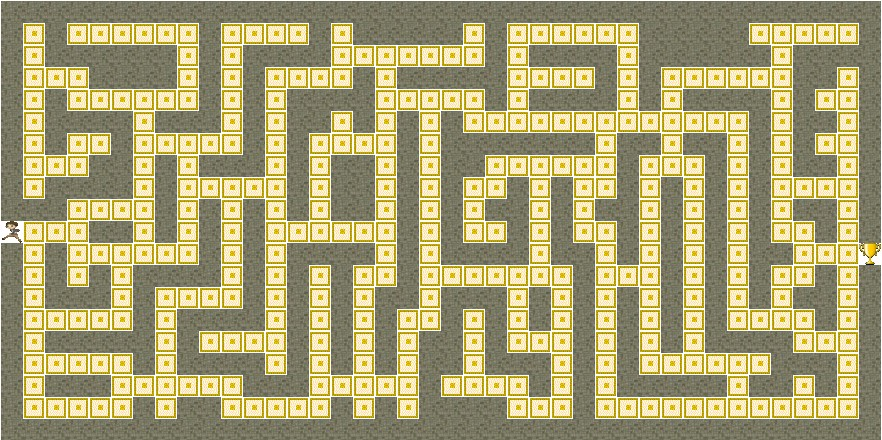
\includegraphics[width=.9\linewidth]{"slikice/labirint.jpg"}
		\label{lab1}
		\caption{Labirint koji se rješava u radu}
	\end{figure}

	S obzirom na to da smo zadan problem smatrali vrlo laganim, odlučili
	smo ga malo proširiti pa smo tako u projektu predstavili i određene
	dodatke koji nisu spominjani nigdje u zadatku. Osim toga su i
	ispravljene tehničke greškice koje su se autorima zadatka podmetnule
	kod opisivanja problema. Vodili smo se srcem u tom slučaju.

    \hypertarget{potraga-za-izgubljenim-blagom-zaboravljenog-faraona}{%
\section{Potraga za izgubljenim blagom zaboravljenog
faraona}\label{potraga-za-izgubljenim-blagom-zaboravljenog-faraona}}

    \hypertarget{baratanje-podatcima}{
\subsection{Baratanje podatcima}\label{baratanje-podatcima}}

Ulazni podaci pohranjeni su u običnoj tekstnoj datoteci u obliku matrice ispunjene nulama i jedinicama pri čemu svaka jedinica predstavlja komadić prohodnog puta u labirintu, a svaka nula je zid kroz koji se ne može proći. Zadani labirint može se iscrtati na sljedeći način:

    \begin{tcolorbox}[breakable, size=fbox, boxrule=1pt, pad at break*=1mm,colback=cellbackground, colframe=cellborder]
\prompt{In}{incolor}{1}{\boxspacing}
\begin{Verbatim}[commandchars=\\\{\}]
\PY{k}{with} \PY{n+nb}{open}\PY{p}{(}\PY{l+s+s2}{\PYZdq{}}\PY{l+s+s2}{data/labirint.txt}\PY{l+s+s2}{\PYZdq{}}\PY{p}{)} \PY{k}{as} \PY{n}{f}\PY{p}{:}
    \PY{k}{for} \PY{n}{x} \PY{o+ow}{in} \PY{n}{f}\PY{o}{.}\PY{n}{readlines}\PY{p}{(}\PY{p}{)}\PY{p}{:}
        \PY{n+nb}{print}\PY{p}{(}\PY{n}{x}\PY{o}{.}\PY{n}{rstrip}\PY{p}{(}\PY{p}{)}\PY{o}{.}\PY{n}{replace}\PY{p}{(}\PY{l+s+s1}{\PYZsq{}}\PY{l+s+s1}{0}\PY{l+s+s1}{\PYZsq{}}\PY{p}{,} \PY{l+s+s1}{\PYZsq{}}\PY{l+s+s1}{  }\PY{l+s+s1}{\PYZsq{}}\PY{p}{)}\PY{o}{.}\PY{n}{replace}\PY{p}{(}\PY{l+s+s1}{\PYZsq{}}\PY{l+s+s1}{1}\PY{l+s+s1}{\PYZsq{}}\PY{p}{,} \PY{l+s+s1}{\PYZsq{}}\PY{l+s+s1}{¤ }\PY{l+s+s1}{\PYZsq{}}\PY{p}{)}\PY{p}{)}
\end{Verbatim}
\end{tcolorbox}

    \begin{Verbatim}[commandchars=\\\{\}]

  ¤   ¤ ¤ ¤ ¤ ¤ ¤   ¤ ¤ ¤ ¤   ¤           ¤   ¤ ¤ ¤ ¤ ¤ ¤           ¤ ¤ ¤ ¤ ¤
  ¤             ¤   ¤         ¤ ¤ ¤ ¤ ¤ ¤ ¤   ¤         ¤             ¤
  ¤ ¤ ¤         ¤   ¤   ¤ ¤ ¤ ¤   ¤           ¤ ¤ ¤ ¤   ¤   ¤ ¤ ¤ ¤ ¤ ¤     ¤
  ¤   ¤ ¤ ¤ ¤ ¤ ¤   ¤   ¤         ¤ ¤ ¤ ¤ ¤   ¤         ¤   ¤         ¤   ¤ ¤
  ¤         ¤       ¤   ¤     ¤   ¤   ¤   ¤ ¤ ¤ ¤ ¤ ¤ ¤ ¤ ¤ ¤ ¤ ¤ ¤   ¤     ¤
  ¤   ¤ ¤   ¤ ¤ ¤ ¤ ¤   ¤   ¤ ¤ ¤ ¤   ¤               ¤     ¤     ¤   ¤   ¤ ¤
  ¤ ¤ ¤     ¤   ¤       ¤   ¤     ¤   ¤     ¤ ¤ ¤ ¤ ¤ ¤   ¤ ¤ ¤   ¤   ¤     ¤
  ¤         ¤   ¤ ¤ ¤ ¤ ¤   ¤     ¤   ¤   ¤ ¤   ¤   ¤ ¤   ¤   ¤   ¤   ¤ ¤ ¤ ¤
      ¤ ¤ ¤ ¤   ¤   ¤   ¤   ¤     ¤   ¤   ¤     ¤   ¤     ¤   ¤   ¤   ¤     ¤
¤ ¤ ¤ ¤     ¤   ¤   ¤   ¤ ¤ ¤ ¤ ¤ ¤   ¤   ¤ ¤   ¤   ¤ ¤   ¤   ¤   ¤   ¤ ¤   ¤
  ¤   ¤ ¤ ¤ ¤ ¤ ¤   ¤   ¤         ¤   ¤         ¤     ¤   ¤   ¤   ¤     ¤ ¤ ¤ ¤
  ¤   ¤   ¤         ¤   ¤   ¤   ¤ ¤   ¤ ¤ ¤ ¤ ¤ ¤ ¤   ¤ ¤ ¤   ¤   ¤   ¤ ¤   ¤
  ¤       ¤   ¤ ¤ ¤ ¤   ¤   ¤   ¤     ¤       ¤   ¤   ¤   ¤   ¤   ¤   ¤     ¤
  ¤ ¤ ¤ ¤ ¤   ¤         ¤   ¤   ¤   ¤ ¤   ¤   ¤   ¤   ¤   ¤   ¤   ¤ ¤ ¤ ¤   ¤
  ¤           ¤   ¤ ¤ ¤ ¤   ¤   ¤   ¤     ¤   ¤ ¤ ¤   ¤   ¤   ¤         ¤ ¤ ¤
  ¤ ¤ ¤ ¤ ¤   ¤         ¤   ¤   ¤   ¤     ¤       ¤   ¤   ¤ ¤ ¤ ¤ ¤ ¤       ¤
  ¤       ¤ ¤ ¤ ¤ ¤ ¤       ¤ ¤ ¤ ¤ ¤   ¤ ¤ ¤ ¤   ¤   ¤           ¤     ¤   ¤
  ¤ ¤ ¤ ¤ ¤   ¤     ¤ ¤ ¤ ¤ ¤   ¤   ¤         ¤ ¤ ¤   ¤ ¤ ¤ ¤ ¤ ¤ ¤ ¤ ¤ ¤ ¤ ¤

    \end{Verbatim}

U datoteci \texttt{vrhovi.txt} pohranjeni su svi vrhovi s pripadajućim koordinatama (redovi i stupci u kojima se pojedini vrhovi nalaze) koji su izračunati pomoću programa \texttt{kreiranje\_grafa} koji je napravljen samo za tu svrhu. Ispod teksta prikazan je ispis prvih 10 vrhova, a u datoteci se nalaze svi.

    \begin{tcolorbox}[breakable, size=fbox, boxrule=1pt, pad at break*=1mm,colback=cellbackground, colframe=cellborder]
\prompt{In}{incolor}{2}{\boxspacing}
\begin{Verbatim}[commandchars=\\\{\}]
\PY{k}{with} \PY{n+nb}{open}\PY{p}{(}\PY{l+s+s2}{\PYZdq{}}\PY{l+s+s2}{data/vrhovi.txt}\PY{l+s+s2}{\PYZdq{}}\PY{p}{)} \PY{k}{as} \PY{n}{f}\PY{p}{:}
    \PY{k}{for} \PY{n}{x} \PY{o+ow}{in} \PY{n}{f}\PY{o}{.}\PY{n}{readlines}\PY{p}{(}\PY{p}{)}\PY{p}{[}\PY{p}{:}\PY{l+m+mi}{10}\PY{p}{]}\PY{p}{:}
        \PY{n+nb}{print}\PY{p}{(}\PY{n}{x}\PY{o}{.}\PY{n}{rstrip}\PY{p}{(}\PY{p}{)}\PY{o}{.}\PY{n}{replace}\PY{p}{(}\PY{l+s+s1}{\PYZsq{}}\PY{l+s+s1}{,}\PY{l+s+s1}{\PYZsq{}}\PY{p}{,} \PY{l+s+s1}{\PYZsq{}}\PY{l+s+se}{\PYZbs{}t}\PY{l+s+s1}{\PYZsq{}}\PY{p}{)}\PY{p}{)}
\end{Verbatim}
\end{tcolorbox}

\begin{samepage}
    \begin{Verbatim}[commandchars=\\\{\}]
naziv   red     stupac
A       10      0
B       10      1
C       10      3
D       9       3
E       9       6
F       6       6
G       6       8
H       6       10
I       1       10
    \end{Verbatim}
\end{samepage}

Nadalje, datoteka \texttt{bridovi.txt} sadrži popis bridova definiranih dvama vrhovima i pripadnom težinom. Slijedi popis prvih 10 bridova.

    \begin{tcolorbox}[breakable, size=fbox, boxrule=1pt, pad at break*=1mm,colback=cellbackground, colframe=cellborder]
\prompt{In}{incolor}{3}{\boxspacing}
\begin{Verbatim}[commandchars=\\\{\}]
\PY{k}{with} \PY{n+nb}{open}\PY{p}{(}\PY{l+s+s2}{\PYZdq{}}\PY{l+s+s2}{data/bridovi.txt}\PY{l+s+s2}{\PYZdq{}}\PY{p}{)} \PY{k}{as} \PY{n}{f}\PY{p}{:}
    \PY{k}{for} \PY{n}{x} \PY{o+ow}{in} \PY{n}{f}\PY{o}{.}\PY{n}{readlines}\PY{p}{(}\PY{p}{)}\PY{p}{[}\PY{p}{:}\PY{l+m+mi}{10}\PY{p}{]}\PY{p}{:}
        \PY{n+nb}{print}\PY{p}{(}\PY{n}{x}\PY{o}{.}\PY{n}{rstrip}\PY{p}{(}\PY{p}{)}\PY{o}{.}\PY{n}{replace}\PY{p}{(}\PY{l+s+s1}{\PYZsq{}}\PY{l+s+s1}{,}\PY{l+s+s1}{\PYZsq{}}\PY{p}{,}\PY{l+s+s1}{\PYZsq{}}\PY{l+s+se}{\PYZbs{}t}\PY{l+s+s1}{\PYZsq{}}\PY{p}{)}\PY{p}{)}
\end{Verbatim}
\end{tcolorbox}

    \begin{Verbatim}[commandchars=\\\{\}]
vrh1    vrh2    tezina
A       B       1
B       C       2
C       D       1
D       E       3
E       F       3
F       G       2
G       H       2
H       I       5
I       J       3
    \end{Verbatim}

    \hypertarget{unos-u-graf}{%
\subsection{Unos u graf}\label{unos-u-graf}}

Za početak, potrebno je napraviti \texttt{import} biblioteka s funkcijama za pretvaranje ulaznih podataka u grafove.

    \begin{tcolorbox}[breakable, size=fbox, boxrule=1pt, pad at break*=1mm,colback=cellbackground, colframe=cellborder]
\prompt{In}{incolor}{4}{\boxspacing}
\begin{Verbatim}[commandchars=\\\{\}]
\PY{k+kn}{from} \PY{n+nn}{scripts} \PY{k+kn}{import} \PY{n}{graf\PYZus{}entry}
\end{Verbatim}
\end{tcolorbox}

Funkcija \texttt{input\_data} pretvara podatke iz ulaznih datoteka u radne podatke o vrhovima, bridovima, početku i kraju labirinta. Funkcija vraća vrhove, bridove, početak i kraj labirinta.

Druga funkcija, \texttt{populate\_graph}, kreira najprije prazan graf, a zatim ga puni bridovima i vrhovima. Ona prima dva argumenta, \texttt{vertices\_names} i \texttt{heuristics}. Prvi prima \texttt{bool} vrijednost (\texttt{True} ili \texttt{False}). Istinita vrijednost prvog argumenta sugerira algoritmu da želimo popularna američka prezimena za imena vrhova, a neistinita da želimo ostaviti slovčane vrijednosti. Ova funkcionalnost nije meritum za dobro izvršavanje algoritma, ali mu da malo duha da nas obična slova ne umore previše. Drugi argument određuje kakva će biti heuristika - ako je on \texttt{sqrt}, heuristika će biti korijen izračunatog broja, a ako je \texttt{pow}, ostat će takav broj kakav je izračunat te će heuristika imati veću težinu s obzirom na prijeđenu udaljenost.

    \begin{tcolorbox}[breakable, size=fbox, boxrule=1pt, pad at break*=1mm,colback=cellbackground, colframe=cellborder]
\prompt{In}{incolor}{5}{\boxspacing}
\begin{Verbatim}[commandchars=\\\{\}]
\PY{n}{graph\PYZus{}data} \PY{o}{=} \PY{n}{graf\PYZus{}entry}\PY{o}{.}\PY{n}{populate\PYZus{}graph}\PY{p}{(}\PY{k+kc}{True}\PY{p}{,} \PY{l+s+s1}{\PYZsq{}}\PY{l+s+s1}{sqrt}\PY{l+s+s1}{\PYZsq{}}\PY{p}{)}
\end{Verbatim}
\end{tcolorbox}

Varijablama se dodjeljuju pripadajuće vrijednosti iz funkcije \texttt{graph\_data}:

    \begin{tcolorbox}[breakable, size=fbox, boxrule=1pt, pad at break*=1mm,colback=cellbackground, colframe=cellborder]
\prompt{In}{incolor}{6}{\boxspacing}
\begin{Verbatim}[commandchars=\\\{\}]
\PY{n}{G} \PY{o}{=} \PY{n}{graph\PYZus{}data}\PY{p}{[}\PY{l+m+mi}{0}\PY{p}{]}
\PY{n}{src} \PY{o}{=} \PY{n}{graph\PYZus{}data}\PY{p}{[}\PY{l+m+mi}{1}\PY{p}{]}
\PY{n}{end} \PY{o}{=} \PY{n}{graph\PYZus{}data}\PY{p}{[}\PY{l+m+mi}{2}\PY{p}{]}
\end{Verbatim}
\end{tcolorbox}

Uvezena je biblioteka \texttt{pprint} kako bi ispis bio uredniji.

    \begin{tcolorbox}[breakable, size=fbox, boxrule=1pt, pad at break*=1mm,colback=cellbackground, colframe=cellborder]
\prompt{In}{incolor}{7}{\boxspacing}
\begin{Verbatim}[commandchars=\\\{\}]
\PY{k+kn}{import} \PY{n+nn}{pprint}
\PY{n}{pp} \PY{o}{=} \PY{n}{pprint}\PY{o}{.}\PY{n}{PrettyPrinter}\PY{p}{(}\PY{p}{)}
\end{Verbatim}
\end{tcolorbox}

Slijedi ispis prvih 10 vrhova iz grafa $G$ s pripadajućim koordinatama.

    \begin{tcolorbox}[breakable, size=fbox, boxrule=1pt, pad at break*=1mm,colback=cellbackground, colframe=cellborder]
\prompt{In}{incolor}{8}{\boxspacing}
\begin{Verbatim}[commandchars=\\\{\}]
\PY{n}{pp}\PY{o}{.}\PY{n}{pprint}\PY{p}{(}\PY{n+nb}{list}\PY{p}{(}\PY{n}{G}\PY{o}{.}\PY{n}{nodes}\PY{p}{(}\PY{n}{data}\PY{o}{=}\PY{l+s+s1}{\PYZsq{}}\PY{l+s+s1}{coords}\PY{l+s+s1}{\PYZsq{}}\PY{p}{)}\PY{p}{)}\PY{p}{[}\PY{p}{:}\PY{l+m+mi}{10}\PY{p}{]}\PY{p}{)}
\end{Verbatim}
\end{tcolorbox}

Nadalje, ispisani su vrhovi iz grafa G s pripadajućim heuristikama. Vrijednosti heuristika dobivene su računanjem "zračne" udaljenosti pojedine točke od točke cilja (duljina hipotenuze prema Pitagorinom poučku).

    \begin{Verbatim}[commandchars=\\\{\}]
[('Smith', ('10', '0')),
 ('Johnson', ('10', '1')),
 ('Williams', ('10', '3')),
 ('Brown', ('9', '3')),
 ('Jones', ('9', '6')),
 ('Miller', ('6', '6')),
 ('Davis', ('6', '8')),
 ('Garcia', ('6', '10')),
 ('Rodriguez', ('1', '10')),
 ('Wilson', ('1', '13'))]
    \end{Verbatim}

    \begin{tcolorbox}[breakable, size=fbox, boxrule=1pt, pad at break*=1mm,colback=cellbackground, colframe=cellborder]
\prompt{In}{incolor}{9}{\boxspacing}
\begin{Verbatim}[commandchars=\\\{\}]
\PY{n}{pp}\PY{o}{.}\PY{n}{pprint}\PY{p}{(}\PY{n+nb}{list}\PY{p}{(}\PY{n}{G}\PY{o}{.}\PY{n}{nodes}\PY{p}{(}\PY{n}{data}\PY{o}{=}\PY{l+s+s1}{\PYZsq{}}\PY{l+s+s1}{h}\PY{l+s+s1}{\PYZsq{}}\PY{p}{)}\PY{p}{)}\PY{p}{[}\PY{p}{:}\PY{l+m+mi}{10}\PY{p}{]}\PY{p}{)}
\end{Verbatim}
\end{tcolorbox}

    \begin{Verbatim}[commandchars=\\\{\}]
[('Smith', 39.01281840626232),
 ('Johnson', 38.01315561749642),
 ('Williams', 36.013886210738214),
 ('Brown', 36.05551275463989),
 ('Jones', 33.06055050963308),
 ('Miller', 33.37663853655727),
 ('Davis', 31.400636936215164),
 ('Garcia', 29.427877939124322),
 ('Rodriguez', 30.675723300355934),
 ('Wilson', 27.85677655436824)]
    \end{Verbatim}


Isto su tako u nastavku ispisani bridovi preko vrhova koje spajaju i s pripadajućim težinama.

    \begin{tcolorbox}[breakable, size=fbox, boxrule=1pt, pad at break*=1mm,colback=cellbackground, colframe=cellborder]
\prompt{In}{incolor}{10}{\boxspacing}
\begin{Verbatim}[commandchars=\\\{\}]
\PY{n}{pp}\PY{o}{.}\PY{n}{pprint}\PY{p}{(}\PY{n+nb}{list}\PY{p}{(}\PY{n}{G}\PY{o}{.}\PY{n}{edges}\PY{p}{(}\PY{n}{data}\PY{o}{=}\PY{l+s+s1}{\PYZsq{}}\PY{l+s+s1}{weight}\PY{l+s+s1}{\PYZsq{}}\PY{p}{)}\PY{p}{)}\PY{p}{[}\PY{p}{:}\PY{l+m+mi}{10}\PY{p}{]}\PY{p}{)}
\end{Verbatim}
\end{tcolorbox}

    \begin{Verbatim}[commandchars=\\\{\}]
[('Smith', 'Johnson', '1'),
 ('Johnson', 'Williams', '2'),
 ('Johnson', 'Gonzales', '4'),
 ('Williams', 'Brown', '1'),
 ('Williams', 'West', '1'),
 ('Brown', 'Jones', '3'),
 ('Jones', 'Miller', '3'),
 ('Jones', 'Wallace', '2'),
 ('Miller', 'Davis', '2'),
 ('Miller', 'Castillo', '2')]
    \end{Verbatim}

Biblioteka \texttt{networkx} koristi se za rad s grafovima. U početku su autori sami pokušali implementirati graf, no ispostavilo se da su koristili vrlo slične strukture podataka kao i \texttt{networkx}, a \texttt{networkx} biblioteka pokazala se kao elegantnije rješenje, a uz to je i testirana pa se vrijeme nije tratilo. Pokušaj implementacije nalazi se u skripti \texttt{graph} u mapi \texttt{scripts}.

    \begin{tcolorbox}[breakable, size=fbox, boxrule=1pt, pad at break*=1mm,colback=cellbackground, colframe=cellborder]
\prompt{In}{incolor}{11}{\boxspacing}
\begin{Verbatim}[commandchars=\\\{\}]
\PY{k+kn}{import} \PY{n+nn}{networkx} \PY{k}{as} \PY{n+nn}{nx}
\end{Verbatim}
\end{tcolorbox}

Naš labirint prikazan je sljedećim grafom. Argumenti funkcije \texttt{draw} su graf $G$ koji se želi nacrtati i izabrani \textit{layout} za prikaz grafa. Osim ovih, mogu se dodati i drugi argumenti za podešavanje pojedinih parametara te je tako ovdje postavljena veličina vrhova na $50\text{px}$.

    \begin{tcolorbox}[breakable, size=fbox, boxrule=1pt, pad at break*=1mm,colback=cellbackground, colframe=cellborder]
\prompt{In}{incolor}{12}{\boxspacing}
\begin{Verbatim}[commandchars=\\\{\}]
\PY{n}{nx}\PY{o}{.}\PY{n}{draw}\PY{p}{(}\PY{n}{G}\PY{p}{,} \PY{n}{nx}\PY{o}{.}\PY{n}{spring\PYZus{}layout}\PY{p}{(}\PY{n}{G}\PY{p}{)}\PY{p}{,} \PY{n}{node\PYZus{}size}\PY{o}{=}\PY{l+m+mi}{50}\PY{p}{)}
\end{Verbatim}
\end{tcolorbox}

    \begin{center}
    \adjustimage{max size={0.9\linewidth}{0.9\paperheight}}{output_14_0.png}
    \end{center}
    { \hspace*{\fill} \\}

    \hypertarget{obiux10dan-graf-bez-prezimena-ljudi}{%
\subsection{Običan graf bez prezimena
ljudi}\label{obiux10dan-graf-bez-prezimena-ljudi}}

U nastavku je prikazan jednak postupak proveden na jednakom grafu uz razliku u imenima vrhova, što je postignuto mijenjanjem prvog pozicijskog argumenta u \texttt{False}.

    \begin{tcolorbox}[breakable, size=fbox, boxrule=1pt, pad at break*=1mm,colback=cellbackground, colframe=cellborder]
\prompt{In}{incolor}{13}{\boxspacing}
\begin{Verbatim}[commandchars=\\\{\}]
\PY{n}{graf\PYZus{}obican} \PY{o}{=} \PY{n}{graf\PYZus{}entry}\PY{o}{.}\PY{n}{populate\PYZus{}graph}\PY{p}{(}\PY{k+kc}{False}\PY{p}{,} \PY{l+s+s1}{\PYZsq{}}\PY{l+s+s1}{sqrt}\PY{l+s+s1}{\PYZsq{}}\PY{p}{)}
\end{Verbatim}
\end{tcolorbox}

    \begin{tcolorbox}[breakable, size=fbox, boxrule=1pt, pad at break*=1mm,colback=cellbackground, colframe=cellborder]
\prompt{In}{incolor}{14}{\boxspacing}
\begin{Verbatim}[commandchars=\\\{\}]
\PY{n}{G\PYZus{}o} \PY{o}{=} \PY{n}{graf\PYZus{}obican}\PY{p}{[}\PY{l+m+mi}{0}\PY{p}{]}
\PY{n}{src\PYZus{}o} \PY{o}{=} \PY{n}{graf\PYZus{}obican}\PY{p}{[}\PY{l+m+mi}{1}\PY{p}{]}
\PY{n}{end\PYZus{}o} \PY{o}{=} \PY{n}{graf\PYZus{}obican}\PY{p}{[}\PY{l+m+mi}{2}\PY{p}{]}
\end{Verbatim}
\end{tcolorbox}

    \begin{tcolorbox}[breakable, size=fbox, boxrule=1pt, pad at break*=1mm,colback=cellbackground, colframe=cellborder]
\prompt{In}{incolor}{15}{\boxspacing}
\begin{Verbatim}[commandchars=\\\{\}]
\PY{n}{pp}\PY{o}{.}\PY{n}{pprint}\PY{p}{(}\PY{n+nb}{list}\PY{p}{(}\PY{n}{G\PYZus{}o}\PY{o}{.}\PY{n}{edges}\PY{p}{(}\PY{n}{data}\PY{o}{=}\PY{l+s+s1}{\PYZsq{}}\PY{l+s+s1}{weight}\PY{l+s+s1}{\PYZsq{}}\PY{p}{)}\PY{p}{)}\PY{p}{[}\PY{p}{:}\PY{l+m+mi}{5}\PY{p}{]}\PY{p}{)}
\end{Verbatim}
\end{tcolorbox}

    \begin{Verbatim}[commandchars=\\\{\}]
[('A', 'B', '1'),
 ('B', 'C', '2'),
 ('B', 'DF', '4'),
 ('C', 'D', '1'),
 ('C', 'DK', '1')]
    \end{Verbatim}

    \begin{tcolorbox}[breakable, size=fbox, boxrule=1pt, pad at break*=1mm,colback=cellbackground, colframe=cellborder]
\prompt{In}{incolor}{16}{\boxspacing}
\begin{Verbatim}[commandchars=\\\{\}]
\PY{n}{pp}\PY{o}{.}\PY{n}{pprint}\PY{p}{(}\PY{n+nb}{list}\PY{p}{(}\PY{n}{G\PYZus{}o}\PY{o}{.}\PY{n}{nodes}\PY{p}{(}\PY{n}{data}\PY{o}{=}\PY{l+s+s1}{\PYZsq{}}\PY{l+s+s1}{coords}\PY{l+s+s1}{\PYZsq{}}\PY{p}{)}\PY{p}{)}\PY{p}{[}\PY{p}{:}\PY{l+m+mi}{5}\PY{p}{]}\PY{p}{)}
\end{Verbatim}
\end{tcolorbox}

    \begin{Verbatim}[commandchars=\\\{\}]
[('A', ('10', '0')),
 ('B', ('10', '1')),
 ('C', ('10', '3')),
 ('D', ('9', '3')),
 ('E', ('9', '6'))]
    \end{Verbatim}

    \hypertarget{smanjivanje-kompleksnosti-grafa}{%
\subsection{Smanjivanje kompleksnosti
grafa}\label{smanjivanje-kompleksnosti-grafa}}

U program se uvozi funkcija \texttt{clean\_graph} iz istoimene skripte koja služi za brisanje nepotrebnih vrhova (i bridova) grafa.

Vrhovi se brišu radi smanjivanja kompleksnosti grafa te tako algoritmima treba kraće vrijeme za izvršavanje, a sam algoritam ne utječe na ispravnost rješenja. Složenost ovog algoritma je $O(n)$, dok Dijkstrin algoritam i \texttt{A*} algoritam imaju kvadratnu složenost pa je ovime ukupno vrijeme izvršavanja kraće.

    \begin{tcolorbox}[breakable, size=fbox, boxrule=1pt, pad at break*=1mm,colback=cellbackground, colframe=cellborder]
\prompt{In}{incolor}{17}{\boxspacing}
\begin{Verbatim}[commandchars=\\\{\}]
\PY{k+kn}{from} \PY{n+nn}{scripts}\PY{n+nn}{.}\PY{n+nn}{clean\PYZus{}graph} \PY{k+kn}{import} \PY{n}{clean\PYZus{}graph}
\end{Verbatim}
\end{tcolorbox}

Funkcija kao argument prima graf kojeg će očistiti. Najprije briše vrhove stupnja 1 jer to znači da je taj vrh završetak slijepe ulice u labirintu i sigurno neće biti dio puta. Ovdje su izuzeti početak i kraj labirinta. Osim toga brišu se i vrhovi stupnja 2 jer su to obični zavoji koji također nemaju utjecaj na put do cilja. Nakon što se vrh stupnja 2 obriše, bridovi koji su ga povezivali s drugim bridovima spajaju se u jedan čija je težina zbroj težina obrisanih bridova.

U kodu ispod funkcija je stavljena u petlju 20 puta jer se autorima to čini optimalno za ovu veličinu grafa. Za veće grafove može se ponoviti i više puta, no nije kritično za izvršavanje programa.

    \begin{tcolorbox}[breakable, size=fbox, boxrule=1pt, pad at break*=1mm,colback=cellbackground, colframe=cellborder]
\prompt{In}{incolor}{18}{\boxspacing}
\begin{Verbatim}[commandchars=\\\{\}]
\PY{n}{cl\PYZus{}graph} \PY{o}{=} \PY{n}{graf\PYZus{}entry}\PY{o}{.}\PY{n}{populate\PYZus{}graph}\PY{p}{(}\PY{k+kc}{True}\PY{p}{,} \PY{l+s+s1}{\PYZsq{}}\PY{l+s+s1}{sqrt}\PY{l+s+s1}{\PYZsq{}}\PY{p}{)}\PY{p}{[}\PY{l+m+mi}{0}\PY{p}{]}

\PY{k}{for} \PY{n}{\PYZus{}} \PY{o+ow}{in} \PY{n+nb}{range}\PY{p}{(}\PY{l+m+mi}{20}\PY{p}{)}\PY{p}{:}
    \PY{n}{cl\PYZus{}graph} \PY{o}{=} \PY{n}{clean\PYZus{}graph}\PY{p}{(}\PY{n}{cl\PYZus{}graph}\PY{p}{,} \PY{n}{src}\PY{p}{,} \PY{n}{end}\PY{p}{)}
\end{Verbatim}
\end{tcolorbox}

Za usporedbu, priložen je ispis brojevnog stanja vrhova grafa prije i poslije čišćenja.

    \begin{tcolorbox}[breakable, size=fbox, boxrule=1pt, pad at break*=1mm,colback=cellbackground, colframe=cellborder]
\prompt{In}{incolor}{19}{\boxspacing}
\begin{Verbatim}[commandchars=\\\{\}]
\PY{n+nb}{print}\PY{p}{(}\PY{l+s+s2}{\PYZdq{}}\PY{l+s+s2}{Cijeli graf: }\PY{l+s+s2}{\PYZdq{}} \PY{o}{+} \PY{n+nb}{str}\PY{p}{(}\PY{n+nb}{len}\PY{p}{(}\PY{n}{G}\PY{o}{.}\PY{n}{edges}\PY{p}{)}\PY{p}{)} \PY{o}{+} \PY{l+s+s2}{\PYZdq{}}\PY{l+s+s2}{ bridova, }\PY{l+s+s2}{\PYZdq{}}\PY{o}{+} \PY{n+nb}{str}\PY{p}{(}\PY{n+nb}{len}\PY{p}{(}\PY{n}{G}\PY{o}{.}\PY{n}{nodes}\PY{p}{)}\PY{p}{)} \PY{o}{+} \PY{l+s+s2}{\PYZdq{}}\PY{l+s+s2}{ vrhova.}\PY{l+s+s2}{\PYZdq{}}\PY{p}{)}
\PY{n+nb}{print}\PY{p}{(}\PY{l+s+s2}{\PYZdq{}}\PY{l+s+s2}{Čisti graf: }\PY{l+s+s2}{\PYZdq{}} \PY{o}{+} \PY{n+nb}{str}\PY{p}{(}\PY{n+nb}{len}\PY{p}{(}\PY{n}{cl\PYZus{}graph}\PY{o}{.}\PY{n}{edges}\PY{p}{)}\PY{p}{)} \PY{o}{+} \PY{l+s+s2}{\PYZdq{}}\PY{l+s+s2}{ bridova, }\PY{l+s+s2}{\PYZdq{}}\PY{o}{+}\PY{n+nb}{str}\PY{p}{(}\PY{n+nb}{len}\PY{p}{(}\PY{n}{cl\PYZus{}graph}\PY{o}{.}\PY{n}{nodes}\PY{p}{)}\PY{p}{)} \PY{o}{+} \PY{l+s+s2}{\PYZdq{}}\PY{l+s+s2}{ vrhova.}\PY{l+s+s2}{\PYZdq{}}\PY{p}{)}
\end{Verbatim}
\end{tcolorbox}

    \begin{Verbatim}[commandchars=\\\{\}]
Cijeli graf: 166 bridova, 147 vrhova.
Čisti graf: 53 bridova, 36 vrhova.
    \end{Verbatim}


Sad je naš labirint značajno pojednostavljen - broj bridova trostruko se
smanjio, a broj se vrhova rasčetvorio. Nije ostao nijedan vrh stupnja 2 ili
manjeg (osim početka i kraja). To se jasno vidi u prikazu pojednostavljenog
grafa:

    \begin{tcolorbox}[breakable, size=fbox, boxrule=1pt, pad at break*=1mm,colback=cellbackground, colframe=cellborder]
\prompt{In}{incolor}{20}{\boxspacing}
\begin{Verbatim}[commandchars=\\\{\}]
\PY{n}{nx}\PY{o}{.}\PY{n}{draw}\PY{p}{(}\PY{n}{cl\PYZus{}graph}\PY{p}{,} \PY{n}{nx}\PY{o}{.}\PY{n}{spring\PYZus{}layout}\PY{p}{(}\PY{n}{cl\PYZus{}graph}\PY{p}{)}\PY{p}{,} \PY{n}{node\PYZus{}size}\PY{o}{=}\PY{l+m+mi}{50}\PY{p}{)}
\end{Verbatim}
\end{tcolorbox}

    \begin{center}
    \adjustimage{max size={0.9\linewidth}{0.9\paperheight}}{output_24_0.png}
    \end{center}
    { \hspace*{\fill} \\}

    \hypertarget{dijkstrin-algoritam}{%
\section{Dijkstrin algoritam}\label{dijkstrin-algoritam}}

Dijkstrin algoritam nećemo previše objašnjavati jer bi on trebao biti dovoljno
jasan iz konteksta kolegija na kojiem se nalazi ovaj projekt.

\subsection{Provedba algoritma}

U program se uvoze funkcije \texttt{RenderTree} i \texttt{Node} iz biblioteke \texttt{anytree} za izradu stabala te funkcija \texttt{dijkstra} iz istoimene skripte koja se nalazi u direktoriju \texttt{scripts}.

    \begin{tcolorbox}[breakable, size=fbox, boxrule=1pt, pad at break*=1mm,colback=cellbackground, colframe=cellborder]
\prompt{In}{incolor}{21}{\boxspacing}
\begin{Verbatim}[commandchars=\\\{\}]
\PY{k+kn}{from} \PY{n+nn}{scripts}\PY{n+nn}{.}\PY{n+nn}{dijkstra} \PY{k+kn}{import} \PY{n}{dijkstra}
\PY{k+kn}{from} \PY{n+nn}{anytree} \PY{k+kn}{import} \PY{n}{RenderTree}\PY{p}{,} \PY{n}{Node}
\end{Verbatim}
\end{tcolorbox}

Algoritam kreće po grafu od ulaza u labirint. Prolazi kroz sve njegove vrhove i računa najkraći put do izlaza iz labirinta. Kad je obišao sve vrhove i pronašao najkraći put, staje s izvođenjem i vraća ga kao rezultat.
Slijedi ispis vrhova kojima prolazi najkraći put prema njihovim imenima te duljina pronađenog najkraćeg puta.

    \begin{tcolorbox}[breakable, size=fbox, boxrule=1pt, pad at break*=1mm,colback=cellbackground, colframe=cellborder]
\prompt{In}{incolor}{22}{\boxspacing}
\begin{Verbatim}[commandchars=\\\{\}]
\PY{n}{distances} \PY{o}{=} \PY{n}{dijkstra}\PY{p}{(}\PY{n}{G}\PY{p}{,} \PY{n}{src}\PY{p}{)}
\PY{n+nb}{print}\PY{p}{(}\PY{l+s+s2}{\PYZdq{}}\PY{l+s+s2}{Put od početka do cilja: }\PY{l+s+s2}{\PYZdq{}}\PY{p}{,} \PY{n+nb}{str}\PY{p}{(}\PY{n}{distances}\PY{p}{[}\PY{l+m+mi}{1}\PY{p}{]}\PY{p}{[}\PY{n}{end}\PY{p}{]}\PY{p}{)}\PY{p}{)}
\PY{n+nb}{print}\PY{p}{(}\PY{l+s+s2}{\PYZdq{}}\PY{l+s+s2}{Broj vrhova u grafovu: }\PY{l+s+s2}{\PYZdq{}} \PY{o}{+} \PY{n+nb}{str}\PY{p}{(}\PY{n+nb}{len}\PY{p}{(}\PY{n}{distances}\PY{p}{[}\PY{l+m+mi}{0}\PY{p}{]}\PY{p}{)}\PY{p}{)}\PY{p}{)}
\end{Verbatim}
\end{tcolorbox}

    \begin{Verbatim}[commandchars=\\\{\}]
Put od početka do cilja:  Node('/Smith/Johnson/Williams/West/Ramos/Wallace/Griff
in/Martinez/Anderson/Taylor/Thomas/Hernandez/Moore/Martin/White/Lopez/Lee/Gonzal
ez/Harris/Clark/Lewis/Robinson/Phillips/Campbell/Ramirez/Scott/Wright/King')
Broj vrhova u grafovu: 147
    \end{Verbatim}

    \begin{tcolorbox}[breakable, size=fbox, boxrule=1pt, pad at break*=1mm,colback=cellbackground, colframe=cellborder]
\prompt{In}{incolor}{23}{\boxspacing}
\begin{Verbatim}[commandchars=\\\{\}]
\PY{n+nb}{print}\PY{p}{(}\PY{l+s+s2}{\PYZdq{}}\PY{l+s+s2}{Najbrži put do cilja dug je }\PY{l+s+s2}{\PYZdq{}} \PY{o}{+} \PY{n+nb}{str}\PY{p}{(}\PY{n}{distances}\PY{p}{[}\PY{l+m+mi}{0}\PY{p}{]}\PY{p}{[}\PY{n}{end}\PY{p}{]}\PY{p}{)} \PY{o}{+} \PY{l+s+s2}{\PYZdq{}}\PY{l+s+s2}{ kvadrata.}\PY{l+s+s2}{\PYZdq{}}\PY{p}{)}
\end{Verbatim}
\end{tcolorbox}

    \begin{Verbatim}[commandchars=\\\{\}]
Najbrži put do cilja dug je 62 kvadrata.
    \end{Verbatim}

    \hypertarget{oux10diux161ux107en-graf---dijkstrin-algoritam}{%
\subsection{Očišćen graf - Dijkstrin
algoritam}\label{oux10diux161ux107en-graf---dijkstrin-algoritam}}

U nastavku je proveden isti algoritam na grafu koji je prethodno pojednostavljen funkcijom \texttt{clean\_graph}.

    \begin{tcolorbox}[breakable, size=fbox, boxrule=1pt, pad at break*=1mm,colback=cellbackground, colframe=cellborder]
\prompt{In}{incolor}{24}{\boxspacing}
\begin{Verbatim}[commandchars=\\\{\}]
\PY{n}{dijkstra\PYZus{}clean\PYZus{}g} \PY{o}{=} \PY{n}{graf\PYZus{}entry}\PY{o}{.}\PY{n}{populate\PYZus{}graph}\PY{p}{(}\PY{k+kc}{True}\PY{p}{,} \PY{l+s+s1}{\PYZsq{}}\PY{l+s+s1}{sqrt}\PY{l+s+s1}{\PYZsq{}}\PY{p}{)}
\PY{n}{dijkstra\PYZus{}clean} \PY{o}{=} \PY{n}{dijkstra\PYZus{}clean\PYZus{}g}\PY{p}{[}\PY{l+m+mi}{0}\PY{p}{]}
\PY{n}{src\PYZus{}clean} \PY{o}{=} \PY{n}{dijkstra\PYZus{}clean\PYZus{}g}\PY{p}{[}\PY{l+m+mi}{1}\PY{p}{]}
\PY{n}{end\PYZus{}clean} \PY{o}{=} \PY{n}{dijkstra\PYZus{}clean\PYZus{}g}\PY{p}{[}\PY{l+m+mi}{2}\PY{p}{]}
\end{Verbatim}
\end{tcolorbox}

Isto kao i prije, funkcija je stavljena u petlju koja se vrti 20 puta.

    \begin{tcolorbox}[breakable, size=fbox, boxrule=1pt, pad at break*=1mm,colback=cellbackground, colframe=cellborder]
\prompt{In}{incolor}{25}{\boxspacing}
\begin{Verbatim}[commandchars=\\\{\}]
\PY{k}{for} \PY{n}{\PYZus{}} \PY{o+ow}{in} \PY{n+nb}{range}\PY{p}{(}\PY{l+m+mi}{20}\PY{p}{)}\PY{p}{:}
    \PY{n}{dijkstra\PYZus{}clean} \PY{o}{=} \PY{n}{clean\PYZus{}graph}\PY{p}{(}\PY{n}{dijkstra\PYZus{}clean}\PY{p}{,} \PY{n}{src\PYZus{}clean}\PY{p}{,} \PY{n}{end\PYZus{}clean}\PY{p}{)}
\end{Verbatim}
\end{tcolorbox}

Sad je graf spreman za provođenje algoritma. Zovemu funkciju za Dijkstrin algoritam kojoj proslijedimo očišćen graf kao argument.

    \begin{tcolorbox}[breakable, size=fbox, boxrule=1pt, pad at break*=1mm,colback=cellbackground, colframe=cellborder]
\prompt{In}{incolor}{26}{\boxspacing}
\begin{Verbatim}[commandchars=\\\{\}]
\PY{n}{distances\PYZus{}clean} \PY{o}{=} \PY{n}{dijkstra}\PY{p}{(}\PY{n}{dijkstra\PYZus{}clean}\PY{p}{,} \PY{n}{src\PYZus{}clean}\PY{p}{)}
\end{Verbatim}
\end{tcolorbox}

Ako se ispišu rezultati nakon provođenja algoritma, put koji se vraća kao najkraći put ima znatno manje vrhova - njih 17. Na prvi se pogled može činiti kao da ovaj niz ima premalo informacija, no zapravo sadrži sve ključne vrhove koji čine najkraći put labirinta zato što između vrhova stupnja 2 koji su bili spajani u algoritmu za čišćenje grafa ionako postoji samo jedan, jedinstveni put.

    \begin{tcolorbox}[breakable, size=fbox, boxrule=1pt, pad at break*=1mm,colback=cellbackground, colframe=cellborder]
\prompt{In}{incolor}{27}{\boxspacing}
\begin{Verbatim}[commandchars=\\\{\}]
\PY{n+nb}{print}\PY{p}{(}\PY{l+s+s2}{\PYZdq{}}\PY{l+s+s2}{Put od početka do cilja: }\PY{l+s+s2}{\PYZdq{}}\PY{p}{,} \PY{n+nb}{str}\PY{p}{(}\PY{n}{distances\PYZus{}clean}\PY{p}{[}\PY{l+m+mi}{1}\PY{p}{]}\PY{p}{[}\PY{n}{end}\PY{p}{]}\PY{p}{)}\PY{p}{)}
\PY{n+nb}{print}\PY{p}{(}\PY{l+s+s2}{\PYZdq{}}\PY{l+s+s2}{Broj vrhova u grafovu: }\PY{l+s+s2}{\PYZdq{}} \PY{o}{+} \PY{n+nb}{str}\PY{p}{(}\PY{n+nb}{len}\PY{p}{(}\PY{n}{distances\PYZus{}clean}\PY{p}{[}\PY{l+m+mi}{0}\PY{p}{]}\PY{p}{)}\PY{p}{)}\PY{p}{)}
\end{Verbatim}
\end{tcolorbox}

    \begin{Verbatim}[commandchars=\\\{\}]
Put od početka do cilja:  Node('/Smith/Johnson/Williams/Ramos/Wallace/Martinez/A
nderson/Taylor/White/Lopez/Harris/Clark/Lewis/Robinson/Ramirez/Wright/King')
Broj vrhova u grafovu: 36
    \end{Verbatim}

Nakon provođenja algoritma na očišćenom grafu, vidi se da je duljina najkraćeg puta identična onoj koja je dobivena provođenjem istog algoritma na originalnom grafu.

    \begin{tcolorbox}[breakable, size=fbox, boxrule=1pt, pad at break*=1mm,colback=cellbackground, colframe=cellborder]
\prompt{In}{incolor}{28}{\boxspacing}
\begin{Verbatim}[commandchars=\\\{\}]
\PY{n+nb}{print}\PY{p}{(}\PY{l+s+s2}{\PYZdq{}}\PY{l+s+s2}{Najbrži put do cilja dug je }\PY{l+s+s2}{\PYZdq{}} \PY{o}{+} \PY{n+nb}{str}\PY{p}{(}\PY{n}{distances\PYZus{}clean}\PY{p}{[}\PY{l+m+mi}{0}\PY{p}{]}\PY{p}{[}\PY{n}{end}\PY{p}{]}\PY{p}{)} \PY{o}{+} \PY{l+s+s2}{\PYZdq{}}\PY{l+s+s2}{ kvadrata.}\PY{l+s+s2}{\PYZdq{}}\PY{p}{)}
\end{Verbatim}
\end{tcolorbox}

    \begin{Verbatim}[commandchars=\\\{\}]
Najbrži put do cilja dug je 62 kvadrata.
    \end{Verbatim}

    \hypertarget{a-algoritam}{%
\section{A* algoritam}\label{a-algoritam}}

U program uvodimo funkciju \texttt{astar} iz istoimene skripte.

    \begin{tcolorbox}[breakable, size=fbox, boxrule=1pt, pad at break*=1mm,colback=cellbackground, colframe=cellborder]
\prompt{In}{incolor}{29}{\boxspacing}
\begin{Verbatim}[commandchars=\\\{\}]
\PY{k+kn}{from} \PY{n+nn}{scripts}\PY{n+nn}{.}\PY{n+nn}{astar} \PY{k+kn}{import} \PY{n}{astar}
\end{Verbatim}
\end{tcolorbox}

\texttt{A*} nalikuje Dijkstrinom algoritmu, no osim težina bridova uzima u
obzir i heuristiku kako bi brže došao do cilja. Heuristika je znanje koja
predočava stvarnu udaljenost nekog vrha od cilja. S obzirom na to da je naš
labirint zadan u obliku matrice, svakom su vrhu točno određene koordinate, pa
se udaljenost od svakog vrha do cilja može lako izračunati.

Najkraća "zračna" udaljenost od vrha do izlaza iz labirinta garantira da nije moguće pronaći put koji je kraći od nje. Algoritam bira idući vrh na sličan način kao Dijkstrin algoritam, samo što neće uzimati u obzir samo udaljenost do idućeg vrha, već će promatrati do sad ukupno prijeđen put i vrijednost heuristike za taj vrh i uzima kao idući vrh onaj čija je vrijednost ukupno najmanja.

Takvo rezoniranje daje tri elementa po kojima se može zaključiti da neki vrh može ili ne može pripadati najkraćem put:
\begin{itemize}
	\item kad je put do cilja pronađen, svaki vrh koji ima heuristiku veću od izračunatog puta ne može biti dio najkraćeg puta
	\item kad je put do cilja izračunat, svaki vrh čiji je zbroj heuristike i put do sebe veći od izračunatog puta do cilja ne može biti dio najkraćeg puta
	\item kad je izračunat put do cilja, svaki vrh do kojeg je put dulji nego izračunat put do cilja ne može pripadati najkraćem putu.
\end{itemize}
Ovim se elementima osigurava da algoritam ne mora proći kroz sve vrhove, već se kontinuirano približava cilju umjesto da traži alternativne puteve na sve strane.

\subsection{Provedba algoritma}

Provedimo algoritam sličnim pozivima kao i Dijkstrin algoritam.

    \begin{tcolorbox}[breakable, size=fbox, boxrule=1pt, pad at break*=1mm,colback=cellbackground, colframe=cellborder]
\prompt{In}{incolor}{30}{\boxspacing}
\begin{Verbatim}[commandchars=\\\{\}]
\PY{n}{distances\PYZus{}a} \PY{o}{=} \PY{n}{astar}\PY{p}{(}\PY{n}{G}\PY{p}{,} \PY{n}{src}\PY{p}{,} \PY{n}{end}\PY{p}{)}
\PY{n+nb}{print}\PY{p}{(}\PY{l+s+s2}{\PYZdq{}}\PY{l+s+s2}{Put od početka do cilja: }\PY{l+s+s2}{\PYZdq{}}\PY{p}{,} \PY{n+nb}{str}\PY{p}{(}\PY{n}{distances\PYZus{}a}\PY{p}{[}\PY{l+m+mi}{1}\PY{p}{]}\PY{p}{[}\PY{n}{end}\PY{p}{]}\PY{p}{)}\PY{p}{)}
\PY{n+nb}{print}\PY{p}{(}\PY{l+s+s2}{\PYZdq{}}\PY{l+s+s2}{Broj vrhova u grafovu: }\PY{l+s+s2}{\PYZdq{}} \PY{o}{+} \PY{n+nb}{str}\PY{p}{(}\PY{n+nb}{len}\PY{p}{(}\PY{n}{distances\PYZus{}a}\PY{p}{[}\PY{l+m+mi}{0}\PY{p}{]}\PY{p}{)}\PY{p}{)}\PY{p}{)}
\end{Verbatim}
\end{tcolorbox}

    \begin{Verbatim}[commandchars=\\\{\}]
Put od početka do cilja:  Node('/Smith/Johnson/Williams/West/Ramos/Wallace/Griff
in/Martinez/Anderson/Taylor/Jenkins/Ortiz/Ross/Morales/White/Lopez/Lee/Gonzalez/
Harris/Clark/Lewis/Robinson/Phillips/Campbell/Ramirez/Scott/Wright/King')
Broj vrhova u grafovu: 147
    \end{Verbatim}

Kao što je ispisano u nastavku, ovaj je algoritam dao jednak rezultat kao i Dijkstrin algoritam u poglavlju iznad.

    \begin{tcolorbox}[breakable, size=fbox, boxrule=1pt, pad at break*=1mm,colback=cellbackground, colframe=cellborder]
\prompt{In}{incolor}{31}{\boxspacing}
\begin{Verbatim}[commandchars=\\\{\}]
\PY{n+nb}{print}\PY{p}{(}\PY{l+s+s2}{\PYZdq{}}\PY{l+s+s2}{Najbrži put do cilja dug je }\PY{l+s+s2}{\PYZdq{}} \PY{o}{+} \PY{n+nb}{str}\PY{p}{(}\PY{n}{distances\PYZus{}a}\PY{p}{[}\PY{l+m+mi}{0}\PY{p}{]}\PY{p}{[}\PY{n}{end}\PY{p}{]}\PY{p}{[}\PY{l+m+mi}{0}\PY{p}{]}\PY{p}{)} \PY{o}{+} \PY{l+s+s2}{\PYZdq{}}\PY{l+s+s2}{ kvadrata.}\PY{l+s+s2}{\PYZdq{}}\PY{p}{)}
\end{Verbatim}
\end{tcolorbox}

    \begin{Verbatim}[commandchars=\\\{\}]
Najbrži put do cilja dug je 62 kvadrata.
    \end{Verbatim}

    \hypertarget{oux10diux161ux107en-graf}{%
\subsection{Očišćen graf}\label{oux10diux161ux107en-graf}}

Kao i u prethodnom poglavlju, funkcija za čišćenje grafa izvršena je i u nastavku u kombinaciji s \texttt{A*} algoritmom. Vrhovima su dodijeljena engleska prezimena kao nazivi, a heuristika svakog vrha bit će korijenovana kako se njena težina ne bi previše naglasila.

    \begin{tcolorbox}[breakable, size=fbox, boxrule=1pt, pad at break*=1mm,colback=cellbackground, colframe=cellborder]
\prompt{In}{incolor}{32}{\boxspacing}
\begin{Verbatim}[commandchars=\\\{\}]
\PY{n}{astar\PYZus{}clean\PYZus{}g} \PY{o}{=} \PY{n}{graf\PYZus{}entry}\PY{o}{.}\PY{n}{populate\PYZus{}graph}\PY{p}{(}\PY{k+kc}{True}\PY{p}{,} \PY{l+s+s1}{\PYZsq{}}\PY{l+s+s1}{sqrt}\PY{l+s+s1}{\PYZsq{}}\PY{p}{)}
\PY{n}{astar\PYZus{}clean} \PY{o}{=} \PY{n}{astar\PYZus{}clean\PYZus{}g}\PY{p}{[}\PY{l+m+mi}{0}\PY{p}{]}
\PY{n}{src\PYZus{}a\PYZus{}clean} \PY{o}{=} \PY{n}{astar\PYZus{}clean\PYZus{}g}\PY{p}{[}\PY{l+m+mi}{1}\PY{p}{]}
\PY{n}{end\PYZus{}a\PYZus{}clean} \PY{o}{=} \PY{n}{astar\PYZus{}clean\PYZus{}g}\PY{p}{[}\PY{l+m+mi}{2}\PY{p}{]}
\end{Verbatim}
\end{tcolorbox}

Kao i prije, funkcija se izvršava 20 puta u petlji.

    \begin{tcolorbox}[breakable, size=fbox, boxrule=1pt, pad at break*=1mm,colback=cellbackground, colframe=cellborder]
\prompt{In}{incolor}{33}{\boxspacing}
\begin{Verbatim}[commandchars=\\\{\}]
\PY{k}{for} \PY{n}{\PYZus{}} \PY{o+ow}{in} \PY{n+nb}{range}\PY{p}{(}\PY{l+m+mi}{20}\PY{p}{)}\PY{p}{:}
    \PY{n}{astar\PYZus{}clean} \PY{o}{=} \PY{n}{clean\PYZus{}graph}\PY{p}{(}\PY{n}{astar\PYZus{}clean}\PY{p}{,} \PY{n}{src\PYZus{}a\PYZus{}clean}\PY{p}{,} \PY{n}{end\PYZus{}a\PYZus{}clean}\PY{p}{)}
\end{Verbatim}
\end{tcolorbox}

Poziva se \texttt{A*} algoritam koji prolazi kroz očišćen graf:

    \begin{tcolorbox}[breakable, size=fbox, boxrule=1pt, pad at break*=1mm,colback=cellbackground, colframe=cellborder]
\prompt{In}{incolor}{34}{\boxspacing}
\begin{Verbatim}[commandchars=\\\{\}]
\PY{n}{distances\PYZus{}a\PYZus{}clean} \PY{o}{=} \PY{n}{astar}\PY{p}{(}\PY{n}{astar\PYZus{}clean}\PY{p}{,} \PY{n}{src\PYZus{}a\PYZus{}clean}\PY{p}{,} \PY{n}{end\PYZus{}a\PYZus{}clean}\PY{p}{)}
\end{Verbatim}
\end{tcolorbox}

Slijedi popis vrhova od ulaza do izlaza iz labirinta te ukupan broj vrhova očišćenog grafa.

    \begin{tcolorbox}[breakable, size=fbox, boxrule=1pt, pad at break*=1mm,colback=cellbackground, colframe=cellborder]
\prompt{In}{incolor}{35}{\boxspacing}
\begin{Verbatim}[commandchars=\\\{\}]
\PY{n+nb}{print}\PY{p}{(}\PY{l+s+s2}{\PYZdq{}}\PY{l+s+s2}{Put od početka do cilja: }\PY{l+s+s2}{\PYZdq{}}\PY{p}{,} \PY{n+nb}{str}\PY{p}{(}\PY{n}{distances\PYZus{}a\PYZus{}clean}\PY{p}{[}\PY{l+m+mi}{1}\PY{p}{]}\PY{p}{[}\PY{n}{end}\PY{p}{]}\PY{p}{)}\PY{p}{)}
\PY{n+nb}{print}\PY{p}{(}\PY{l+s+s2}{\PYZdq{}}\PY{l+s+s2}{Broj vrhova u grafovu: }\PY{l+s+s2}{\PYZdq{}} \PY{o}{+} \PY{n+nb}{str}\PY{p}{(}\PY{n+nb}{len}\PY{p}{(}\PY{n}{distances\PYZus{}a\PYZus{}clean}\PY{p}{[}\PY{l+m+mi}{0}\PY{p}{]}\PY{p}{)}\PY{p}{)}\PY{p}{)}
\end{Verbatim}
\end{tcolorbox}

    \begin{Verbatim}[commandchars=\\\{\}]
Put od početka do cilja:  Node('/Smith/Johnson/Williams/Ramos/Wallace/Martinez/A
nderson/Taylor/White/Lopez/Harris/Clark/Lewis/Robinson/Ramirez/Wright/King')
Broj vrhova u grafovu: 36
    \end{Verbatim}

Rezultat je ponovno jednak kao prije - duljina je najkraćeg puta 62.

    \begin{tcolorbox}[breakable, size=fbox, boxrule=1pt, pad at break*=1mm,colback=cellbackground, colframe=cellborder]
\prompt{In}{incolor}{36}{\boxspacing}
\begin{Verbatim}[commandchars=\\\{\}]
\PY{n+nb}{print}\PY{p}{(}\PY{l+s+s2}{\PYZdq{}}\PY{l+s+s2}{Najbrži put do cilja dug je }\PY{l+s+s2}{\PYZdq{}} \PY{o}{+} \PY{n+nb}{str}\PY{p}{(}\PY{n}{distances\PYZus{}clean}\PY{p}{[}\PY{l+m+mi}{0}\PY{p}{]}\PY{p}{[}\PY{n}{end}\PY{p}{]}\PY{p}{)} \PY{o}{+} \PY{l+s+s2}{\PYZdq{}}\PY{l+s+s2}{ kvadrata.}\PY{l+s+s2}{\PYZdq{}}\PY{p}{)}
\end{Verbatim}
\end{tcolorbox}

    \begin{Verbatim}[commandchars=\\\{\}]
Najbrži put do cilja dug je 62 kvadrata.
    \end{Verbatim}

    \hypertarget{heuristika-koja-ne-uzima-korijen-iz-udaljenosti}{%
\subsection{Heuristika koja ne uzima korijen iz
udaljenosti}\label{heuristika-koja-ne-uzima-korijen-iz-udaljenosti}}

Demonstracije radi, u nastavku je izvršen \texttt{A*} algoritam koji ne korijenuje heuristiku, već zadržava kvadratne vrijednosti. Ovo ima negativan učinak na krajnji rezultat zato što previše važnosti daje vrijednosti heuristike u odnosu na prijeđenu udaljenost, što može rezultirati neoptimalnim putem.

    \begin{tcolorbox}[breakable, size=fbox, boxrule=1pt, pad at break*=1mm,colback=cellbackground, colframe=cellborder]
\prompt{In}{incolor}{37}{\boxspacing}
\begin{Verbatim}[commandchars=\\\{\}]
\PY{n}{graph\PYZus{}pow} \PY{o}{=} \PY{n}{graf\PYZus{}entry}\PY{o}{.}\PY{n}{populate\PYZus{}graph}\PY{p}{(}\PY{k+kc}{True}\PY{p}{,} \PY{l+s+s1}{\PYZsq{}}\PY{l+s+s1}{pow}\PY{l+s+s1}{\PYZsq{}}\PY{p}{)}
\end{Verbatim}
\end{tcolorbox}

Ovdje nije uzet očišćen, već originalni graf te je algoritam izvršen na njemu.

    \begin{tcolorbox}[breakable, size=fbox, boxrule=1pt, pad at break*=1mm,colback=cellbackground, colframe=cellborder]
\prompt{In}{incolor}{38}{\boxspacing}
\begin{Verbatim}[commandchars=\\\{\}]
\PY{n}{G\PYZus{}a} \PY{o}{=} \PY{n}{graph\PYZus{}pow}\PY{p}{[}\PY{l+m+mi}{0}\PY{p}{]}
\PY{n}{src\PYZus{}a} \PY{o}{=} \PY{n}{graph\PYZus{}pow}\PY{p}{[}\PY{l+m+mi}{1}\PY{p}{]}
\PY{n}{end\PYZus{}a} \PY{o}{=} \PY{n}{graph\PYZus{}pow}\PY{p}{[}\PY{l+m+mi}{2}\PY{p}{]}
\end{Verbatim}
\end{tcolorbox}

Kao rezultat, vraćen je drukčiji put nego što je bio kad su vrijednosti heuristika bile korijenovane.

    \begin{tcolorbox}[breakable, size=fbox, boxrule=1pt, pad at break*=1mm,colback=cellbackground, colframe=cellborder]
\prompt{In}{incolor}{39}{\boxspacing}
\begin{Verbatim}[commandchars=\\\{\}]
\PY{n}{distances\PYZus{}a\PYZus{}pow} \PY{o}{=} \PY{n}{astar}\PY{p}{(}\PY{n}{G\PYZus{}a}\PY{p}{,} \PY{n}{src\PYZus{}a}\PY{p}{,} \PY{n}{end\PYZus{}a}\PY{p}{)}
\PY{n+nb}{print}\PY{p}{(}\PY{l+s+s2}{\PYZdq{}}\PY{l+s+s2}{Put od početka do cilja: }\PY{l+s+s2}{\PYZdq{}}\PY{p}{,} \PY{n+nb}{str}\PY{p}{(}\PY{n}{distances\PYZus{}a\PYZus{}pow}\PY{p}{[}\PY{l+m+mi}{1}\PY{p}{]}\PY{p}{[}\PY{n}{end}\PY{p}{]}\PY{p}{)}\PY{p}{)}
\PY{n+nb}{print}\PY{p}{(}\PY{l+s+s2}{\PYZdq{}}\PY{l+s+s2}{Broj vrhova u grafovu: }\PY{l+s+s2}{\PYZdq{}} \PY{o}{+} \PY{n+nb}{str}\PY{p}{(}\PY{n+nb}{len}\PY{p}{(}\PY{n}{distances\PYZus{}a\PYZus{}pow}\PY{p}{[}\PY{l+m+mi}{0}\PY{p}{]}\PY{p}{)}\PY{p}{)}\PY{p}{)}
\end{Verbatim}
\end{tcolorbox}

    \begin{Verbatim}[commandchars=\\\{\}]
Put od početka do cilja:  Node('/Smith/Johnson/Williams/Brown/Jones/Miller/Davis
/Martinez/Anderson/Taylor/Thomas/Hernandez/Moore/Martin/White/Lopez/Lee/Gonzalez
/Harris/Clark/Lewis/Robinson/Phillips/Campbell/Ramirez/Evans/Turner/Torres/Wrigh
t/King')
Broj vrhova u grafovu: 147
    \end{Verbatim}

Učinak se jasno vidi kod ispisa duljine "najkraćeg" puta, koji u ovom slučaju zapravo nije najkraći. Algoritam ovdje vraća put koji je za dvije jedinice dulji nego u svim dosadašnjim rješenjima.

Ovisno o vrsti, veličini i strukturi labirinta ili postavljenim prioritetima, heuristika koju koristi \texttt{A*} ne mora uvijek biti korijen iz zbroja kvadrata udaljenosti promatrane točke i točke cilja po osi ordinata i apscisa. Ovdje se to pokazalo kao dobro rješenje, između ostalog zato što je graf relativno malen, no dovoljno kompleksan da svaki algoritam za njegovo rješavanje nije jednako učinkovit, te zato što je on prikazan matrično, odnosno struktura grafa pogoduje za ovakav način rješavanja. Zaključuje se da se heuristika odabire i koristi u skladu sa zahtjevima problema koji se rješava ovim algoritmom.

    \begin{tcolorbox}[breakable, size=fbox, boxrule=1pt, pad at break*=1mm,colback=cellbackground, colframe=cellborder]
\prompt{In}{incolor}{40}{\boxspacing}
\begin{Verbatim}[commandchars=\\\{\}]
\PY{n+nb}{print}\PY{p}{(}\PY{l+s+s2}{\PYZdq{}}\PY{l+s+s2}{Najbrži put do cilja dug je }\PY{l+s+s2}{\PYZdq{}} \PY{o}{+} \PY{n+nb}{str}\PY{p}{(}\PY{n}{distances\PYZus{}a\PYZus{}pow}\PY{p}{[}\PY{l+m+mi}{0}\PY{p}{]}\PY{p}{[}\PY{n}{end}\PY{p}{]}\PY{p}{[}\PY{l+m+mi}{0}\PY{p}{]}\PY{p}{)} \PY{o}{+} \PY{l+s+s2}{\PYZdq{}}\PY{l+s+s2}{ kvadrata.}\PY{l+s+s2}{\PYZdq{}}\PY{p}{)}
\end{Verbatim}
\end{tcolorbox}

    \begin{Verbatim}[commandchars=\\\{\}]
Najbrži put do cilja dug je 64 kvadrata.
    \end{Verbatim}

    \hypertarget{usporedba-rjeux161enja-algoritama}{%
\section{Usporedba rješenja
algoritama}\label{usporedba-rjeux161enja-algoritama}}

U nastavku su rezimirani rezultati provedbe algoritama s pojedinim modifikacijama.

U prvoj je usporedbi vidljiva suptilna razlika u konkretnom putu koji je vraćen kao najkraći u ova dva algoritma, no duljina im je na kraju jednaka.

    \begin{tcolorbox}[breakable, size=fbox, boxrule=1pt, pad at break*=1mm,colback=cellbackground, colframe=cellborder]
\prompt{In}{incolor}{41}{\boxspacing}
\begin{Verbatim}[commandchars=\\\{\}]
\PY{c+c1}{\PYZsh{} dijkstra}
\PY{n}{pp}\PY{o}{.}\PY{n}{pprint}\PY{p}{(}\PY{n}{distances}\PY{p}{[}\PY{l+m+mi}{1}\PY{p}{]}\PY{p}{[}\PY{n}{end}\PY{p}{]}\PY{p}{)}
\PY{c+c1}{\PYZsh{} astar}
\PY{n}{pp}\PY{o}{.}\PY{n}{pprint}\PY{p}{(}\PY{n}{distances\PYZus{}a}\PY{p}{[}\PY{l+m+mi}{1}\PY{p}{]}\PY{p}{[}\PY{n}{end}\PY{p}{]}\PY{p}{)}
\end{Verbatim}
\end{tcolorbox}

    \begin{Verbatim}[commandchars=\\\{\}]
Node('/Smith/Johnson/Williams/West/Ramos/Wallace/Griffin/Martinez/Anderson/Taylo
r/Thomas/Hernandez/Moore/Martin/White/Lopez/Lee/Gonzalez/Harris/Clark/Lewis/Robi
nson/Phillips/Campbell/Ramirez/Scott/Wright/King')
Node('/Smith/Johnson/Williams/West/Ramos/Wallace/Griffin/Martinez/Anderson/Taylo
r/Jenkins/Ortiz/Ross/Morales/White/Lopez/Lee/Gonzalez/Harris/Clark/Lewis/Robinso
n/Phillips/Campbell/Ramirez/Scott/Wright/King')
    \end{Verbatim}

Kad su se isti algoritmi provodili na očišćenim verzijama grafa labirinta, rješenje je ispalo identično u oba slučaja.

    \begin{tcolorbox}[breakable, size=fbox, boxrule=1pt, pad at break*=1mm,colback=cellbackground, colframe=cellborder]
\prompt{In}{incolor}{42}{\boxspacing}
\begin{Verbatim}[commandchars=\\\{\}]
\PY{c+c1}{\PYZsh{} dijkstra ociscen}
\PY{n}{pp}\PY{o}{.}\PY{n}{pprint}\PY{p}{(}\PY{n}{distances\PYZus{}clean}\PY{p}{[}\PY{l+m+mi}{1}\PY{p}{]}\PY{p}{[}\PY{n}{end}\PY{p}{]}\PY{p}{)}
\PY{c+c1}{\PYZsh{} astar ociscen}
\PY{n}{pp}\PY{o}{.}\PY{n}{pprint}\PY{p}{(}\PY{n}{distances\PYZus{}a\PYZus{}clean}\PY{p}{[}\PY{l+m+mi}{1}\PY{p}{]}\PY{p}{[}\PY{n}{end}\PY{p}{]}\PY{p}{)}
\end{Verbatim}
\end{tcolorbox}

    \begin{Verbatim}[commandchars=\\\{\}]
Node('/Smith/Johnson/Williams/Ramos/Wallace/Martinez/Anderson/Taylor/White/Lopez
/Harris/Clark/Lewis/Robinson/Ramirez/Wright/King')
Node('/Smith/Johnson/Williams/Ramos/Wallace/Martinez/Anderson/Taylor/White/Lopez
/Harris/Clark/Lewis/Robinson/Ramirez/Wright/King')
    \end{Verbatim}

U posljednjoj usporedbi vidi se očita razlika u rezultatu, što je prouzročeno pogrešnim odabirom heuristike. Tako je put nepotrebno dulji jer je u postupku odabran pogrešan prioritet te je u ovom slučaju Dijkstrin algoritam zapravo vratio bolji rezultat nego \texttt{A*} zbog nepreciznog provođenja.

    \begin{tcolorbox}[breakable, size=fbox, boxrule=1pt, pad at break*=1mm,colback=cellbackground, colframe=cellborder]
\prompt{In}{incolor}{43}{\boxspacing}
\begin{Verbatim}[commandchars=\\\{\}]
\PY{c+c1}{\PYZsh{} astar \PYZhy{} dobra heuristika}
\PY{n}{pp}\PY{o}{.}\PY{n}{pprint}\PY{p}{(}\PY{n}{distances\PYZus{}a\PYZus{}clean}\PY{p}{[}\PY{l+m+mi}{1}\PY{p}{]}\PY{p}{[}\PY{n}{end}\PY{p}{]}\PY{p}{)}
\PY{c+c1}{\PYZsh{} astar \PYZhy{} \PYZsq{}pretjerana\PYZsq{} heuristika}
\PY{n}{pp}\PY{o}{.}\PY{n}{pprint}\PY{p}{(}\PY{n}{distances\PYZus{}a\PYZus{}pow}\PY{p}{[}\PY{l+m+mi}{1}\PY{p}{]}\PY{p}{[}\PY{n}{end}\PY{p}{]}\PY{p}{)}
\end{Verbatim}
\end{tcolorbox}

    \begin{Verbatim}[commandchars=\\\{\}]
Node('/Smith/Johnson/Williams/Ramos/Wallace/Martinez/Anderson/Taylor/White/Lopez
/Harris/Clark/Lewis/Robinson/Ramirez/Wright/King')
Node('/Smith/Johnson/Williams/Brown/Jones/Miller/Davis/Martinez/Anderson/Taylor/
Thomas/Hernandez/Moore/Martin/White/Lopez/Lee/Gonzalez/Harris/Clark/Lewis/Robins
on/Phillips/Campbell/Ramirez/Evans/Turner/Torres/Wright/King')
    \end{Verbatim}

\section{Zaključak}

Ovaj je rad imao u cilju demonstrirati dva algoritma koja služe za pronalazak
puta kroz labirint. Naglasak je napravljen na njihovim razlikama te prednostima
i nedostatcima. I Dijkstra i \texttt{A*} algoritmi nam garantiraju siguran
dolazak do cilja, no Dijkstrin algoritam ima određene nedostatke koji se jako
manifestiraju na ogromnim grafovima, odnosno labirintima. Njih \texttt{A*}
izbjegava koristeći heuristike te tako puno manje vrhova obrađuje nego što bi
to napravio Dijkstra, a pritom očuva vjerodostojnost rezultata.

Usporediti algoritme se može na mnoge načine, a mnogi od njih nisu posve očiti.
Složenost obaju algoritama je ista, no \texttt{A*} na puno sofisticiraniji
način traži smjer u kojem pronalaziti put do cilja. Osim toga, \texttt{A*}
algoritam gotovo pola vrhova uopće nije morao pregledavati jer su mu heuristike
dopustile da ih ignorira.

Na temu heuristika treba i napomenuti kako je važan odabir heuristika kako bi
rezultat bio dovoljno dobar. Premale vrijednosti heuristika mogu dovesti do
usporavanja algoritma i gubitka prednosti koje nam donosi \texttt{A*}, dok
previsoke vrijednosti mogu dovesti do krivih rezultata jer premalen utjecaj ima
put koji je prijeđen do neke točke.

Osim algoritama, ovaj se težak problem može brže riješiti prilagodbom grafa
tako da se eliminiraju nepotrebni bridovi i vrhovi kroz koje se sigurno neće
prolaziti. Na konkretnom se primjeru u ovom zadatku broj vrhova smanjio više od
četiri puta, a broj bridova više od tri puta.

Ispravnim pristupom i teški se problemi mogu jednostavno riješiti i ovaj rad je
imao za cilj demonstrirati eleganciju i jednostavnost rješavanja ovog teškog
problema.

%    \hypertarget{appendix}{%
%\section{Appendix}\label{appendix}}

%    \hypertarget{prikaz-stabla-putova}{%
%\subsection{Prikaz stabla putova}\label{prikaz-stabla-putova}}

%    \hypertarget{dijkstrin-algoritam}{%
%\subsubsection{Dijkstrin algoritam}\label{dijkstrin-algoritam}}

%    \begin{tcolorbox}[breakable, size=fbox, boxrule=1pt, pad at break*=1mm,colback=cellbackground, colframe=cellborder]
%\prompt{In}{incolor}{44}{\boxspacing}
%\begin{Verbatim}[commandchars=\\\{\}]
%\PY{k}{for} \PY{n}{pre}\PY{p}{,} \PY{n}{fill}\PY{p}{,} \PY{n}{node} \PY{o+ow}{in} \PY{n}{RenderTree}\PY{p}{(}\PY{n}{distances}\PY{p}{[}\PY{l+m+mi}{1}\PY{p}{]}\PY{p}{[}\PY{n}{src}\PY{p}{]}\PY{p}{)}\PY{p}{:}
%    \PY{n+nb}{print}\PY{p}{(}\PY{n}{pre} \PY{o}{+} \PY{n}{node}\PY{o}{.}\PY{n}{name}\PY{p}{)}
%\end{Verbatim}
%\end{tcolorbox}
%
%    \begin{Verbatim}[commandchars=\\\{\}]
%Smith
%└── Johnson
%    ├── Williams
%    │   ├── Brown
%    │   │   └── Jones
%    │   │       └── Miller
%    │   │           ├── Davis
%    │   │           │   └── Garcia
%    │   │           │       └── Rodriguez
%    │   │           │           └── Wilson
%    │   │           └── Castillo
%    │   │               ├── Olson
%    │   │               │   └── Webb
%    │   │               │       └── Washington
%    │   │               └── Tucker
%    │   │                   └── Freeman
%    │   │                       └── Burns
%    │   │                           ├── Henry
%    │   │                           └── Vasquez
%    │   │                               ├── Snyder
%    │   │                               │   └── Simpson
%    │   │                               │       └── Crawford
%    │   │                               └── Jimenez
%    │   └── West
%    │       ├── Ramos
%    │       │   └── Wallace
%    │       │       └── Griffin
%    │       │           └── Martinez
%    │       │               └── Anderson
%    │       │                   ├── Taylor
%    │       │                   │   ├── Thomas
%    │       │                   │   │   └── Hernandez
%    │       │                   │   │       └── Moore
%    │       │                   │   │           ├── Martin
%    │       │                   │   │           │   ├── Jackson
%    │       │                   │   │           │   │   └── Thompson
%    │       │                   │   │           │   └── White
%    │       │                   │   │           │       └── Lopez
%    │       │                   │   │           │           └── Lee
%    │       │                   │   │           │               └── Gonzalez
%    │       │                   │   │           │                   └── Harris
%    │       │                   │   │           │                       ├──
%Clark
%    │       │                   │   │           │                       │   ├──
%Lewis
%    │       │                   │   │           │                       │   │
%└── Robinson
%    │       │                   │   │           │                       │   │
%├── Walker
%    │       │                   │   │           │                       │   │
%│   └── Perez
%    │       │                   │   │           │                       │   │
%│       └── Hall
%    │       │                   │   │           │                       │   │
%│           ├── Young
%    │       │                   │   │           │                       │   │
%│           │   └── Allen
%    │       │                   │   │           │                       │   │
%│           │       └── Sanchez
%    │       │                   │   │           │                       │   │
%│           │           └── Edwards
%    │       │                   │   │           │                       │   │
%│           └── Collins
%    │       │                   │   │           │                       │   │
%├── Phillips
%    │       │                   │   │           │                       │   │
%│   └── Campbell
%    │       │                   │   │           │                       │   │
%│       ├── Ramirez
%    │       │                   │   │           │                       │   │
%│       │   ├── Scott
%    │       │                   │   │           │                       │   │
%│       │   │   ├── Wright
%    │       │                   │   │           │                       │   │
%│       │   │   │   └── King
%    │       │                   │   │           │                       │   │
%│       │   │   └── Green
%    │       │                   │   │           │                       │   │
%│       │   │       ├── Baker
%    │       │                   │   │           │                       │   │
%│       │   │       │   ├── Adams
%    │       │                   │   │           │                       │   │
%│       │   │       │   └── Nelson
%    │       │                   │   │           │                       │   │
%│       │   │       └── Hill
%    │       │                   │   │           │                       │   │
%│       │   └── Evans
%    │       │                   │   │           │                       │   │
%│       │       └── Turner
%    │       │                   │   │           │                       │   │
%│       │           └── Torres
%    │       │                   │   │           │                       │   │
%│       │               └── Parker
%    │       │                   │   │           │                       │   │
%│       └── Mitchell
%    │       │                   │   │           │                       │   │
%│           ├── Roberts
%    │       │                   │   │           │                       │   │
%│           └── Carter
%    │       │                   │   │           │                       │   │
%└── Rogers
%    │       │                   │   │           │                       │   │
%├── Cook
%    │       │                   │   │           │                       │   │
%│   └── Rivera
%    │       │                   │   │           │                       │   │
%│       └── Nguyen
%    │       │                   │   │           │                       │   │
%│           ├── Morris
%    │       │                   │   │           │                       │   │
%│           │   └── Stewart
%    │       │                   │   │           │                       │   │
%│           │       └── Flores
%    │       │                   │   │           │                       │   │
%│           └── Murphy
%    │       │                   │   │           │                       │   │
%└── Morgan
%    │       │                   │   │           │                       │   │
%└── Peterson
%    │       │                   │   │           │                       │   │
%└── Ruiz
%    │       │                   │   │           │                       │   └──
%Kelly
%    │       │                   │   │           │                       │
%├── Gomez
%    │       │                   │   │           │                       │
%│   └── Bell
%    │       │                   │   │           │                       │
%│       └── Bailey
%    │       │                   │   │           │                       │
%│           └── Reed
%    │       │                   │   │           │                       │
%│               └── Cooper
%    │       │                   │   │           │                       │
%│                   └── Harrison
%    │       │                   │   │           │                       │
%└── Howard
%    │       │                   │   │           │                       └──
%Alvarez
%    │       │                   │   │           │                           ├──
%Wells
%    │       │                   │   │           │                           │
%└── Kennedy
%    │       │                   │   │           │                           └──
%Woods
%    │       │                   │   │           └── Mendoza
%    │       │                   │   └── Jenkins
%    │       │                   │       ├── Ortiz
%    │       │                   │       │   ├── Ross
%    │       │                   │       │   │   ├── Sanders
%    │       │                   │       │   │   │   └── Foster
%    │       │                   │       │   │   └── Morales
%    │       │                   │       │   └── Russell
%    │       │                   │       │       └── Powell
%    │       │                   │       │           └── Sullivan
%    │       │                   │       └── Gutierrez
%    │       │                   │           ├── Perry
%    │       │                   │           └── Butler
%    │       │                   └── Reynolds
%    │       └── Cole
%    └── Gonzales
%        ├── Kim
%        │   ├── Graham
%        │   │   └── Hamilton
%        │   │       └── Patterson
%        │   │           ├── Simmons
%        │   │           │   └── Coleman
%        │   │           │       └── Henderson
%        │   │           │           └── Barnes
%        │   │           │               ├── Long
%        │   │           │               │   ├── Myers
%        │   │           │               │   │   ├── Price
%        │   │           │               │   │   │   └── Hughes
%        │   │           │               │   │   │       └── Cruz
%        │   │           │               │   │   │           └── Reyes
%        │   │           │               │   │   │               ├── Brooks
%        │   │           │               │   │   │               │   ├── Ward
%        │   │           │               │   │   │               │   │   └── Cox
%        │   │           │               │   │   │               │   │       └──
%Diaz
%        │   │           │               │   │   │               │   │
%└── Richardson
%        │   │           │               │   │   │               │   │
%└── Wood
%        │   │           │               │   │   │               │   │
%└── Watson
%        │   │           │               │   │   │               │   └── Bennett
%        │   │           │               │   │   │               │       └── Gray
%        │   │           │               │   │   │               │           └──
%Stevens
%        │   │           │               │   │   │               │
%└── Murray
%        │   │           │               │   │   │               │
%└── Ford
%        │   │           │               │   │   │               │
%└── Marshall
%        │   │           │               │   │   │               │
%├── Owens
%        │   │           │               │   │   │               │
%└── Mcdonald
%        │   │           │               │   │   │               └── James
%        │   │           │               │   │   └── Ellis
%        │   │           │               │   └── Bryant
%        │   │           │               └── Fisher
%        │   │           ├── Jordan
%        │   │           └── Gibson
%        │   └── Hayes
%        │       └── Chavez
%        └── Alexander
%    \end{Verbatim}
%
%    \hypertarget{oux10diux161ux107en-dijkstrin-algoritam}{%
%\subsubsection{Očišćen Dijkstrin
%algoritam}\label{oux10diux161ux107en-dijkstrin-algoritam}}
%
%    \begin{tcolorbox}[breakable, size=fbox, boxrule=1pt, pad at break*=1mm,colback=cellbackground, colframe=cellborder]
%\prompt{In}{incolor}{45}{\boxspacing}
%\begin{Verbatim}[commandchars=\\\{\}]
%\PY{k}{for} \PY{n}{pre}\PY{p}{,} \PY{n}{fill}\PY{p}{,} \PY{n}{node} \PY{o+ow}{in} \PY{n}{RenderTree}\PY{p}{(}\PY{n}{distances\PYZus{}clean}\PY{p}{[}\PY{l+m+mi}{1}\PY{p}{]}\PY{p}{[}\PY{n}{src}\PY{p}{]}\PY{p}{)}\PY{p}{:}
%    \PY{n+nb}{print}\PY{p}{(}\PY{n}{pre} \PY{o}{+} \PY{n}{node}\PY{o}{.}\PY{n}{name}\PY{p}{)}
%\end{Verbatim}
%\end{tcolorbox}
%
%    \begin{Verbatim}[commandchars=\\\{\}]
%Smith
%└── Johnson
%    ├── Williams
%    │   ├── Jones
%    │   └── Ramos
%    │       └── Wallace
%    │           └── Martinez
%    │               └── Anderson
%    │                   └── Taylor
%    │                       ├── White
%    │                       │   └── Lopez
%    │                       │       └── Harris
%    │                       │           └── Clark
%    │                       │               ├── Lewis
%    │                       │               │   └── Robinson
%    │                       │               │       ├── Hall
%    │                       │               │       │   └── Sanchez
%    │                       │               │       ├── Ramirez
%    │                       │               │       │   ├── Wright
%    │                       │               │       │   │   └── King
%    │                       │               │       │   └── Torres
%    │                       │               │       └── Rogers
%    │                       │               │           ├── Rivera
%    │                       │               │           │   └── Morris
%    │                       │               │           └── Peterson
%    │                       │               └── Kelly
%    │                       │                   ├── Bell
%    │                       │                   │   └── Cooper
%    │                       │                   └── Howard
%    │                       └── Ortiz
%    │                           ├── Ross
%    │                           └── Morales
%    └── Gonzales
%        └── Patterson
%            └── Long
%                └── Cruz
%    \end{Verbatim}
%
%    \hypertarget{a-algoritam}{%
%\subsubsection{A* algoritam}\label{a-algoritam}}
%
%    \begin{tcolorbox}[breakable, size=fbox, boxrule=1pt, pad at break*=1mm,colback=cellbackground, colframe=cellborder]
%\prompt{In}{incolor}{46}{\boxspacing}
%\begin{Verbatim}[commandchars=\\\{\}]
%\PY{k}{for} \PY{n}{pre}\PY{p}{,} \PY{n}{fill}\PY{p}{,} \PY{n}{node} \PY{o+ow}{in} \PY{n}{RenderTree}\PY{p}{(}\PY{n}{distances\PYZus{}a}\PY{p}{[}\PY{l+m+mi}{1}\PY{p}{]}\PY{p}{[}\PY{n}{src}\PY{p}{]}\PY{p}{)}\PY{p}{:}
%    \PY{n+nb}{print}\PY{p}{(}\PY{n}{pre} \PY{o}{+} \PY{n}{node}\PY{o}{.}\PY{n}{name}\PY{p}{)}
%\end{Verbatim}
%\end{tcolorbox}
%
%    \begin{Verbatim}[commandchars=\\\{\}]
%Smith
%└── Johnson
%    ├── Williams
%    │   ├── Brown
%    │   │   └── Jones
%    │   │       └── Miller
%    │   │           ├── Davis
%    │   │           │   └── Garcia
%    │   │           │       └── Rodriguez
%    │   │           │           └── Wilson
%    │   │           └── Castillo
%    │   │               ├── Olson
%    │   │               │   └── Webb
%    │   │               │       └── Washington
%    │   │               └── Tucker
%    │   │                   └── Freeman
%    │   │                       └── Burns
%    │   │                           ├── Henry
%    │   │                           └── Vasquez
%    │   │                               ├── Snyder
%    │   │                               │   └── Simpson
%    │   │                               │       └── Crawford
%    │   │                               └── Jimenez
%    │   └── West
%    │       ├── Ramos
%    │       │   ├── Alexander
%    │       │   └── Wallace
%    │       │       └── Griffin
%    │       │           └── Martinez
%    │       │               └── Anderson
%    │       │                   ├── Taylor
%    │       │                   │   ├── Thomas
%    │       │                   │   │   └── Hernandez
%    │       │                   │   │       └── Moore
%    │       │                   │   │           ├── Martin
%    │       │                   │   │           │   ├── Jackson
%    │       │                   │   │           │   │   └── Thompson
%    │       │                   │   │           │   └── White
%    │       │                   │   │           │       └── Lopez
%    │       │                   │   │           │           └── Lee
%    │       │                   │   │           │               └── Gonzalez
%    │       │                   │   │           │                   └── Harris
%    │       │                   │   │           │                       ├──
%Clark
%    │       │                   │   │           │                       │   ├──
%Lewis
%    │       │                   │   │           │                       │   │
%└── Robinson
%    │       │                   │   │           │                       │   │
%├── Walker
%    │       │                   │   │           │                       │   │
%│   └── Perez
%    │       │                   │   │           │                       │   │
%│       └── Hall
%    │       │                   │   │           │                       │   │
%│           ├── Young
%    │       │                   │   │           │                       │   │
%│           │   └── Allen
%    │       │                   │   │           │                       │   │
%│           │       └── Sanchez
%    │       │                   │   │           │                       │   │
%│           └── Collins
%    │       │                   │   │           │                       │   │
%│               └── Parker
%    │       │                   │   │           │                       │   │
%├── Phillips
%    │       │                   │   │           │                       │   │
%│   └── Campbell
%    │       │                   │   │           │                       │   │
%│       ├── Ramirez
%    │       │                   │   │           │                       │   │
%│       │   ├── Scott
%    │       │                   │   │           │                       │   │
%│       │   │   └── Green
%    │       │                   │   │           │                       │   │
%│       │   │       ├── Baker
%    │       │                   │   │           │                       │   │
%│       │   │       │   ├── Adams
%    │       │                   │   │           │                       │   │
%│       │   │       │   └── Nelson
%    │       │                   │   │           │                       │   │
%│       │   │       └── Hill
%    │       │                   │   │           │                       │   │
%│       │   └── Evans
%    │       │                   │   │           │                       │   │
%│       │       └── Turner
%    │       │                   │   │           │                       │   │
%│       │           └── Torres
%    │       │                   │   │           │                       │   │
%│       │               └── Wright
%    │       │                   │   │           │                       │   │
%│       │                   └── King
%    │       │                   │   │           │                       │   │
%│       └── Mitchell
%    │       │                   │   │           │                       │   │
%│           ├── Roberts
%    │       │                   │   │           │                       │   │
%│           └── Carter
%    │       │                   │   │           │                       │   │
%└── Rogers
%    │       │                   │   │           │                       │   │
%├── Cook
%    │       │                   │   │           │                       │   │
%│   └── Rivera
%    │       │                   │   │           │                       │   │
%│       └── Nguyen
%    │       │                   │   │           │                       │   │
%│           ├── Morris
%    │       │                   │   │           │                       │   │
%│           │   └── Stewart
%    │       │                   │   │           │                       │   │
%│           └── Murphy
%    │       │                   │   │           │                       │   │
%└── Morgan
%    │       │                   │   │           │                       │   │
%└── Peterson
%    │       │                   │   │           │                       │   │
%└── Ruiz
%    │       │                   │   │           │                       │   └──
%Kelly
%    │       │                   │   │           │                       │
%├── Gomez
%    │       │                   │   │           │                       │
%└── Howard
%    │       │                   │   │           │                       │
%└── Bell
%    │       │                   │   │           │                       │
%└── Bailey
%    │       │                   │   │           │                       │
%└── Reed
%    │       │                   │   │           │                       │
%└── Cooper
%    │       │                   │   │           │                       │
%└── Harrison
%    │       │                   │   │           │                       └──
%Alvarez
%    │       │                   │   │           │                           ├──
%Wells
%    │       │                   │   │           │                           │
%└── Kennedy
%    │       │                   │   │           │                           └──
%Woods
%    │       │                   │   │           └── Mendoza
%    │       │                   │   └── Jenkins
%    │       │                   │       ├── Ortiz
%    │       │                   │       │   ├── Ross
%    │       │                   │       │   │   └── Sanders
%    │       │                   │       │   │       └── Foster
%    │       │                   │       │   └── Russell
%    │       │                   │       │       └── Powell
%    │       │                   │       │           ├── Morales
%    │       │                   │       │           └── Sullivan
%    │       │                   │       └── Gutierrez
%    │       │                   │           ├── Perry
%    │       │                   │           └── Butler
%    │       │                   └── Reynolds
%    │       └── Cole
%    └── Gonzales
%        └── Kim
%            ├── Graham
%            │   └── Hamilton
%            │       └── Patterson
%            │           ├── Simmons
%            │           │   └── Coleman
%            │           │       └── Henderson
%            │           │           └── Barnes
%            │           │               ├── Long
%            │           │               │   ├── Myers
%            │           │               │   │   ├── Price
%            │           │               │   │   │   └── Hughes
%            │           │               │   │   │       └── Cruz
%            │           │               │   │   │           └── Reyes
%            │           │               │   │   │               ├── Brooks
%            │           │               │   │   │               │   ├── Ward
%            │           │               │   │   │               │   │   └── Cox
%            │           │               │   │   │               │   │       └──
%Diaz
%            │           │               │   │   │               │   │
%└── Richardson
%            │           │               │   │   │               │   │
%└── Wood
%            │           │               │   │   │               │   │
%└── Watson
%            │           │               │   │   │               │   └── Bennett
%            │           │               │   │   │               │       └── Gray
%            │           │               │   │   │               │           └──
%Stevens
%            │           │               │   │   │               │
%└── Murray
%            │           │               │   │   │               │
%└── Ford
%            │           │               │   │   │               │
%└── Marshall
%            │           │               │   │   │               │
%├── Owens
%            │           │               │   │   │               │
%└── Mcdonald
%            │           │               │   │   │               └── James
%            │           │               │   │   └── Ellis
%            │           │               │   └── Bryant
%            │           │               └── Fisher
%            │           ├── Jordan
%            │           └── Gibson
%            └── Hayes
%                └── Chavez
%    \end{Verbatim}
%
%    \hypertarget{a-algoritam-s-pretjeranom-heuristikom}{%
%\subsubsection{A* algoritam s pretjeranom
%heuristikom}\label{a-algoritam-s-pretjeranom-heuristikom}}
%
%    \begin{tcolorbox}[breakable, size=fbox, boxrule=1pt, pad at break*=1mm,colback=cellbackground, colframe=cellborder]
%\prompt{In}{incolor}{47}{\boxspacing}
%\begin{Verbatim}[commandchars=\\\{\}]
%\PY{k}{for} \PY{n}{pre}\PY{p}{,} \PY{n}{fill}\PY{p}{,} \PY{n}{node} \PY{o+ow}{in} \PY{n}{RenderTree}\PY{p}{(}\PY{n}{distances\PYZus{}a\PYZus{}pow}\PY{p}{[}\PY{l+m+mi}{1}\PY{p}{]}\PY{p}{[}\PY{n}{src}\PY{p}{]}\PY{p}{)}\PY{p}{:}
%    \PY{n+nb}{print}\PY{p}{(}\PY{n}{pre} \PY{o}{+} \PY{n}{node}\PY{o}{.}\PY{n}{name}\PY{p}{)}
%\end{Verbatim}
%\end{tcolorbox}
%
%    \begin{Verbatim}[commandchars=\\\{\}]
%Smith
%└── Johnson
%    ├── Williams
%    │   ├── Brown
%    │   │   └── Jones
%    │   │       └── Miller
%    │   │           ├── Davis
%    │   │           │   ├── Garcia
%    │   │           │   │   └── Rodriguez
%    │   │           │   │       └── Wilson
%    │   │           │   └── Martinez
%    │   │           │       └── Anderson
%    │   │           │           ├── Taylor
%    │   │           │           │   ├── Thomas
%    │   │           │           │   │   └── Hernandez
%    │   │           │           │   │       └── Moore
%    │   │           │           │   │           ├── Martin
%    │   │           │           │   │           │   ├── Jackson
%    │   │           │           │   │           │   │   └── Thompson
%    │   │           │           │   │           │   └── White
%    │   │           │           │   │           │       └── Lopez
%    │   │           │           │   │           │           ├── Lee
%    │   │           │           │   │           │           │   └── Gonzalez
%    │   │           │           │   │           │           │       └── Harris
%    │   │           │           │   │           │           │           ├──
%Clark
%    │   │           │           │   │           │           │           │   ├──
%Lewis
%    │   │           │           │   │           │           │           │   │
%└── Robinson
%    │   │           │           │   │           │           │           │   │
%├── Walker
%    │   │           │           │   │           │           │           │   │
%│   └── Perez
%    │   │           │           │   │           │           │           │   │
%│       └── Hall
%    │   │           │           │   │           │           │           │   │
%│           ├── Young
%    │   │           │           │   │           │           │           │   │
%│           │   └── Allen
%    │   │           │           │   │           │           │           │   │
%│           │       └── Sanchez
%    │   │           │           │   │           │           │           │   │
%│           └── Collins
%    │   │           │           │   │           │           │           │   │
%├── Phillips
%    │   │           │           │   │           │           │           │   │
%│   └── Campbell
%    │   │           │           │   │           │           │           │   │
%│       ├── Ramirez
%    │   │           │           │   │           │           │           │   │
%│       │   ├── Scott
%    │   │           │           │   │           │           │           │   │
%│       │   │   └── Green
%    │   │           │           │   │           │           │           │   │
%│       │   │       ├── Baker
%    │   │           │           │   │           │           │           │   │
%│       │   │       │   ├── Adams
%    │   │           │           │   │           │           │           │   │
%│       │   │       │   └── Nelson
%    │   │           │           │   │           │           │           │   │
%│       │   │       └── Hill
%    │   │           │           │   │           │           │           │   │
%│       │   └── Evans
%    │   │           │           │   │           │           │           │   │
%│       │       └── Turner
%    │   │           │           │   │           │           │           │   │
%│       │           └── Torres
%    │   │           │           │   │           │           │           │   │
%│       │               ├── Wright
%    │   │           │           │   │           │           │           │   │
%│       │               │   └── King
%    │   │           │           │   │           │           │           │   │
%│       │               └── Parker
%    │   │           │           │   │           │           │           │   │
%│       └── Mitchell
%    │   │           │           │   │           │           │           │   │
%│           ├── Roberts
%    │   │           │           │   │           │           │           │   │
%│           └── Carter
%    │   │           │           │   │           │           │           │   │
%└── Rogers
%    │   │           │           │   │           │           │           │   │
%├── Cook
%    │   │           │           │   │           │           │           │   │
%│   └── Rivera
%    │   │           │           │   │           │           │           │   │
%│       └── Nguyen
%    │   │           │           │   │           │           │           │   │
%│           ├── Morris
%    │   │           │           │   │           │           │           │   │
%│           │   └── Stewart
%    │   │           │           │   │           │           │           │   │
%│           └── Murphy
%    │   │           │           │   │           │           │           │   │
%└── Morgan
%    │   │           │           │   │           │           │           │   │
%└── Peterson
%    │   │           │           │   │           │           │           │   │
%└── Ruiz
%    │   │           │           │   │           │           │           │   └──
%Kelly
%    │   │           │           │   │           │           │           │
%└── Gomez
%    │   │           │           │   │           │           │           └──
%Alvarez
%    │   │           │           │   │           │           │               ├──
%Wells
%    │   │           │           │   │           │           │               │
%└── Kennedy
%    │   │           │           │   │           │           │               └──
%Woods
%    │   │           │           │   │           │           └── Cruz
%    │   │           │           │   │           │               ├── Reyes
%    │   │           │           │   │           │               │   ├── Brooks
%    │   │           │           │   │           │               │   │   ├── Ward
%    │   │           │           │   │           │               │   │   │   ├──
%Howard
%    │   │           │           │   │           │               │   │   │   │
%└── Bell
%    │   │           │           │   │           │               │   │   │   │
%└── Bailey
%    │   │           │           │   │           │               │   │   │   │
%└── Reed
%    │   │           │           │   │           │               │   │   │   │
%└── Cooper
%    │   │           │           │   │           │               │   │   │   │
%└── Harrison
%    │   │           │           │   │           │               │   │   │   └──
%Cox
%    │   │           │           │   │           │               │   │   │
%└── Diaz
%    │   │           │           │   │           │               │   │   │
%└── Richardson
%    │   │           │           │   │           │               │   │   │
%└── Wood
%    │   │           │           │   │           │               │   │   │
%└── Watson
%    │   │           │           │   │           │               │   │   └──
%Bennett
%    │   │           │           │   │           │               │   └── James
%    │   │           │           │   │           │               │       └── Gray
%    │   │           │           │   │           │               │           └──
%Stevens
%    │   │           │           │   │           │               │
%└── Murray
%    │   │           │           │   │           │               │
%└── Ford
%    │   │           │           │   │           │               │
%└── Marshall
%    │   │           │           │   │           │               │
%├── Owens
%    │   │           │           │   │           │               │
%└── Mcdonald
%    │   │           │           │   │           │               └── Hughes
%    │   │           │           │   │           │                   └── Price
%    │   │           │           │   │           └── Mendoza
%    │   │           │           │   └── Jenkins
%    │   │           │           │       ├── Ortiz
%    │   │           │           │       │   ├── Ross
%    │   │           │           │       │   │   └── Sanders
%    │   │           │           │       │   │       └── Foster
%    │   │           │           │       │   └── Russell
%    │   │           │           │       │       └── Powell
%    │   │           │           │       │           ├── Morales
%    │   │           │           │       │           └── Sullivan
%    │   │           │           │       └── Gutierrez
%    │   │           │           │           ├── Perry
%    │   │           │           │           └── Butler
%    │   │           │           └── Reynolds
%    │   │           │               └── Jordan
%    │   │           └── Castillo
%    │   │               ├── Olson
%    │   │               │   └── Webb
%    │   │               │       └── Washington
%    │   │               └── Tucker
%    │   │                   └── Freeman
%    │   │                       └── Burns
%    │   │                           ├── Henry
%    │   │                           └── Vasquez
%    │   │                               ├── Snyder
%    │   │                               │   └── Simpson
%    │   │                               │       └── Crawford
%    │   │                               └── Jimenez
%    │   └── West
%    │       ├── Ramos
%    │       │   ├── Alexander
%    │       │   └── Wallace
%    │       │       └── Griffin
%    │       └── Cole
%    └── Gonzales
%        └── Kim
%            ├── Graham
%            │   └── Hamilton
%            │       ├── Patterson
%            │       │   ├── Simmons
%            │       │   │   └── Coleman
%            │       │   │       └── Henderson
%            │       │   │           └── Barnes
%            │       │   │               ├── Long
%            │       │   │               │   ├── Myers
%            │       │   │               │   │   └── Ellis
%            │       │   │               │   └── Bryant
%            │       │   │               └── Fisher
%            │       │   └── Gibson
%            │       └── Chavez
%            └── Hayes
%    \end{Verbatim}
%
%
%    % Add a bibliography block to the postdoc
%
%

\end{document}
